% Options for packages loaded elsewhere
\PassOptionsToPackage{unicode}{hyperref}
\PassOptionsToPackage{hyphens}{url}
\PassOptionsToPackage{dvipsnames,svgnames*,x11names*}{xcolor}
%
\documentclass[
  12pt,
]{book}
\usepackage{amsmath,amssymb}
\usepackage{lmodern}
\usepackage{setspace}
\usepackage{ifxetex,ifluatex}
\ifnum 0\ifxetex 1\fi\ifluatex 1\fi=0 % if pdftex
  \usepackage[T1]{fontenc}
  \usepackage[utf8]{inputenc}
  \usepackage{textcomp} % provide euro and other symbols
\else % if luatex or xetex
  \usepackage{unicode-math}
  \defaultfontfeatures{Scale=MatchLowercase}
  \defaultfontfeatures[\rmfamily]{Ligatures=TeX,Scale=1}
\fi
% Use upquote if available, for straight quotes in verbatim environments
\IfFileExists{upquote.sty}{\usepackage{upquote}}{}
\IfFileExists{microtype.sty}{% use microtype if available
  \usepackage[]{microtype}
  \UseMicrotypeSet[protrusion]{basicmath} % disable protrusion for tt fonts
}{}
\makeatletter
\@ifundefined{KOMAClassName}{% if non-KOMA class
  \IfFileExists{parskip.sty}{%
    \usepackage{parskip}
  }{% else
    \setlength{\parindent}{0pt}
    \setlength{\parskip}{6pt plus 2pt minus 1pt}}
}{% if KOMA class
  \KOMAoptions{parskip=half}}
\makeatother
\usepackage{xcolor}
\IfFileExists{xurl.sty}{\usepackage{xurl}}{} % add URL line breaks if available
\IfFileExists{bookmark.sty}{\usepackage{bookmark}}{\usepackage{hyperref}}
\hypersetup{
  pdftitle={Estudio Longitudinal Social de Chile},
  colorlinks=true,
  linkcolor=blue,
  filecolor=Maroon,
  citecolor=Blue,
  urlcolor=Blue,
  pdfcreator={LaTeX via pandoc}}
\urlstyle{same} % disable monospaced font for URLs
\usepackage[left=4cm, right=3cm, top=2.5cm, bottom=2.5cm]{geometry}
\usepackage{color}
\usepackage{fancyvrb}
\newcommand{\VerbBar}{|}
\newcommand{\VERB}{\Verb[commandchars=\\\{\}]}
\DefineVerbatimEnvironment{Highlighting}{Verbatim}{commandchars=\\\{\}}
% Add ',fontsize=\small' for more characters per line
\usepackage{framed}
\definecolor{shadecolor}{RGB}{248,248,248}
\newenvironment{Shaded}{\begin{snugshade}}{\end{snugshade}}
\newcommand{\AlertTok}[1]{\textcolor[rgb]{0.94,0.16,0.16}{#1}}
\newcommand{\AnnotationTok}[1]{\textcolor[rgb]{0.56,0.35,0.01}{\textbf{\textit{#1}}}}
\newcommand{\AttributeTok}[1]{\textcolor[rgb]{0.77,0.63,0.00}{#1}}
\newcommand{\BaseNTok}[1]{\textcolor[rgb]{0.00,0.00,0.81}{#1}}
\newcommand{\BuiltInTok}[1]{#1}
\newcommand{\CharTok}[1]{\textcolor[rgb]{0.31,0.60,0.02}{#1}}
\newcommand{\CommentTok}[1]{\textcolor[rgb]{0.56,0.35,0.01}{\textit{#1}}}
\newcommand{\CommentVarTok}[1]{\textcolor[rgb]{0.56,0.35,0.01}{\textbf{\textit{#1}}}}
\newcommand{\ConstantTok}[1]{\textcolor[rgb]{0.00,0.00,0.00}{#1}}
\newcommand{\ControlFlowTok}[1]{\textcolor[rgb]{0.13,0.29,0.53}{\textbf{#1}}}
\newcommand{\DataTypeTok}[1]{\textcolor[rgb]{0.13,0.29,0.53}{#1}}
\newcommand{\DecValTok}[1]{\textcolor[rgb]{0.00,0.00,0.81}{#1}}
\newcommand{\DocumentationTok}[1]{\textcolor[rgb]{0.56,0.35,0.01}{\textbf{\textit{#1}}}}
\newcommand{\ErrorTok}[1]{\textcolor[rgb]{0.64,0.00,0.00}{\textbf{#1}}}
\newcommand{\ExtensionTok}[1]{#1}
\newcommand{\FloatTok}[1]{\textcolor[rgb]{0.00,0.00,0.81}{#1}}
\newcommand{\FunctionTok}[1]{\textcolor[rgb]{0.00,0.00,0.00}{#1}}
\newcommand{\ImportTok}[1]{#1}
\newcommand{\InformationTok}[1]{\textcolor[rgb]{0.56,0.35,0.01}{\textbf{\textit{#1}}}}
\newcommand{\KeywordTok}[1]{\textcolor[rgb]{0.13,0.29,0.53}{\textbf{#1}}}
\newcommand{\NormalTok}[1]{#1}
\newcommand{\OperatorTok}[1]{\textcolor[rgb]{0.81,0.36,0.00}{\textbf{#1}}}
\newcommand{\OtherTok}[1]{\textcolor[rgb]{0.56,0.35,0.01}{#1}}
\newcommand{\PreprocessorTok}[1]{\textcolor[rgb]{0.56,0.35,0.01}{\textit{#1}}}
\newcommand{\RegionMarkerTok}[1]{#1}
\newcommand{\SpecialCharTok}[1]{\textcolor[rgb]{0.00,0.00,0.00}{#1}}
\newcommand{\SpecialStringTok}[1]{\textcolor[rgb]{0.31,0.60,0.02}{#1}}
\newcommand{\StringTok}[1]{\textcolor[rgb]{0.31,0.60,0.02}{#1}}
\newcommand{\VariableTok}[1]{\textcolor[rgb]{0.00,0.00,0.00}{#1}}
\newcommand{\VerbatimStringTok}[1]{\textcolor[rgb]{0.31,0.60,0.02}{#1}}
\newcommand{\WarningTok}[1]{\textcolor[rgb]{0.56,0.35,0.01}{\textbf{\textit{#1}}}}
\usepackage{longtable,booktabs,array}
\usepackage{calc} % for calculating minipage widths
% Correct order of tables after \paragraph or \subparagraph
\usepackage{etoolbox}
\makeatletter
\patchcmd\longtable{\par}{\if@noskipsec\mbox{}\fi\par}{}{}
\makeatother
% Allow footnotes in longtable head/foot
\IfFileExists{footnotehyper.sty}{\usepackage{footnotehyper}}{\usepackage{footnote}}
\makesavenoteenv{longtable}
\usepackage{graphicx}
\makeatletter
\def\maxwidth{\ifdim\Gin@nat@width>\linewidth\linewidth\else\Gin@nat@width\fi}
\def\maxheight{\ifdim\Gin@nat@height>\textheight\textheight\else\Gin@nat@height\fi}
\makeatother
% Scale images if necessary, so that they will not overflow the page
% margins by default, and it is still possible to overwrite the defaults
% using explicit options in \includegraphics[width, height, ...]{}
\setkeys{Gin}{width=\maxwidth,height=\maxheight,keepaspectratio}
% Set default figure placement to htbp
\makeatletter
\def\fps@figure{htbp}
\makeatother
\setlength{\emergencystretch}{3em} % prevent overfull lines
\providecommand{\tightlist}{%
  \setlength{\itemsep}{0pt}\setlength{\parskip}{0pt}}
\setcounter{secnumdepth}{5}
\usepackage{booktabs}
\usepackage{booktabs}
\usepackage{longtable}
\usepackage{array}
\usepackage{multirow}
\usepackage{wrapfig}
\usepackage{float}
\usepackage{colortbl}
\usepackage{pdflscape}
\usepackage{tabu}
\usepackage{threeparttable}
\usepackage{threeparttablex}
\usepackage[normalem]{ulem}
\usepackage{makecell}
\usepackage{xcolor}
\ifluatex
  \usepackage{selnolig}  % disable illegal ligatures
\fi

\title{Estudio Longitudinal Social de Chile}
\usepackage{etoolbox}
\makeatletter
\providecommand{\subtitle}[1]{% add subtitle to \maketitle
  \apptocmd{\@title}{\par {\large #1 \par}}{}{}
}
\makeatother
\subtitle{Resultados longitudinales 2016-2021}
\author{}
\date{\vspace{-2.5em}2021-11-24}

\begin{document}
\maketitle

{
\hypersetup{linkcolor=}
\setcounter{tocdepth}{1}
\tableofcontents
}
\listoftables
\listoffigures
\setstretch{1.5}
\hypertarget{introduccion}{%
\chapter{Introduccion}\label{introduccion}}

El Centro de Estudios de Conflicto y Cohesión Social (\href{https://coes.cl/}{COES}) tiene el agrado de publicar el informe ``Radiografía del Cambio Social,'' el cual consolida los principales hallazgos longitudinales de cinco mediciones anuales del Estudio Longitudinal Social de Chile (\href{https://coes.cl/encuesta-panel/}{ELSOC}).

ELSOC es una encuesta desarrollada para analizar longitudinalmente, en un estudio panel, la evolución del conflicto y cohesión social en la sociedad chilena, basándose en modelos conceptuales descritos en la literatura nacional e internacional de las disciplinas del ámbito de la Economía, Sociología, Psicología, Ciencia Política y Estudios Urbanos. De este modo, se orienta a examinar los principales antecedentes, factores moderadores y mediadores, así como las principales consecuencias asociadas al desarrollo de distintas formas de sociabilidad en Chile.

Desde 2019 y hasta la fecha, Chile se ha visto remecido por importantes eventos que han alterado aspectos sociales, políticos y económicos de la vida nacional: la pandemia asociada al COVID-19, y las consecuencias del estallido social más grande de las últimas décadas, ocurrido a partir de octubre de 2019, el que ha desencadenado un proceso constituyente inédito en la historia de Chile.

Ambos fenómenos han significado un desafío para ELSOC, ya que afecta tanto la forma en que son levantados los datos, como las preguntas que el estudio debe abordar. Sin embargo, ELSOC presente una gran oportunidad única: la posibilidad de observar el efecto que éstos fenómenos tienen sobre la población chilena desde una perspectiva longitudinal.

\hypertarget{sobre-coes}{%
\section{Sobre COES}\label{sobre-coes}}

El Centro de Estudios de Conflicto y Cohesión Social (\href{https://coes.cl/}{COES}) desarrolla investigación colaborativa en temas relacionados al conflicto social y la cohesión (convivencia) en Chile, por medio de un equipo multidisciplinario proveniente de las ciencias sociales y humanidades. COES centra sus actividades académicas y de difusión en el análisis de las múltiples manifestaciones del conflicto y cohesión social en Chile, sus causas, así como también su contexto cultural e histórico.

COES está patrocinado por la Universidad de Chile y la Pontificia Universidad Católica de Chile, y como instituciones asociadas se encuentran la Universidad Diego Portales y la Universidad Adolfo Ibáñez. COES cuenta con el apoyo del Fondo de Financiamiento de Centros de Investigación en Áreas Prioritarias (\href{https://www.conicyt.cl/fondap/sobre-fondap/que-es-fondap/}{FONDAP}, dependiente de la Agencia Nacional de Investigación y Desarrollo (\href{https://www.anid.cl/}{ANID}) del Ministerio de Ciencia, Tecnología, Conocimiento e Innovación (\href{https://www.minciencia.gob.cl/}{MinCiencia}). ELSOC además cuenta como socio al Instituto Milenio para la Investigación en Depresión y Personalidad (\href{https://midap.org/}{MIDAP}).

\hypertarget{sobre-elsoc}{%
\section{Sobre ELSOC}\label{sobre-elsoc}}

\hypertarget{descripciuxf3n-del-estudio}{%
\subsection{Descripción del estudio}\label{descripciuxf3n-del-estudio}}

El \href{https://coes.cl/encuesta-panel/}{Estudio Longitudinal Social de Chile (ELSOC)} es una encuesta panel, representativa de la población nacional urbana, que analiza la estabilidad y cambio de las creencias, actitudes y percepciones que tenemos los chilenos y chilenas respecto de la convivencia y del conflicto, la cohesión y una amplia gama de aspectos políticos y sociales a lo largo del tiempo.

Este estudio sigue la evolución de cerca de 4.500 chilenos y chilenas a lo largo de una década. Actualmente se encuentran disponibles 5 olas del estudio, abarcando el período entre 2016 y 2021. Sus temas de estudio y su aspecto longitudinal convierten a ELSOC en un recurso único en Chile y América Latina para analizar la evolución de la sociedad chilena y para el desarrollo de las ciencias sociales en Chile.

Durante los últimos años, ELSOC se ha consolidado como un importante insumo para el desarrollo de investigación científica y aplicada en ciencias sociales. En el sitio web de (ELSOC)(\url{https://coes.cl/encuesta-panel/}) se puede acceder a más información sobre el estudio.

\hypertarget{acceso-a-bases-de-datos-elsoc}{%
\subsection{Acceso a Bases de Datos ELSOC}\label{acceso-a-bases-de-datos-elsoc}}

Las bases de datos y documentación correspondientes se encuentran disponibles, de manera libre y gratuita, en un repositorio de datos, al cual se podrá acceder en el link:

\url{https://dataverse.harvard.edu/dataverse/elsoc}

En este sitio se obtendrá acceso a los datos de las 5 mediciones transversales de ELSOC, así como bases longitudinales que integran las distintas mediciones. En colaboración con el Centro de Inteligencia Territorial (\href{https://cit.uai.cl/}{CIT}), se pone también a disposición las bases ELSOC-CIT. Estas bases de datos permiten combinar la información de ELSOC, y estimaciones e indicadores territoriales y geoespaciales de distinta índole, proveniente de diversas fuentes de información nacional para los períodos 2016 a 2019.

ELSOC tiene un compromiso con los más altos estándares científicos en términos de producción y análisis de datos. Dentro de esta visión global, ELSOC se guía por las principales pautas de Transparencia y Apertura en la investigación científica. Por esta misma razón, los códigos utilizados para el desarrollo de este documento se encontrarán disponibles en \url{https://github.com/centro-coes}.

\hypertarget{caracteruxedsticas-del-diseuxf1o-muestral}{%
\subsection{Características del diseño muestral}\label{caracteruxedsticas-del-diseuxf1o-muestral}}

\begin{itemize}
\item
  Unidad de Análisis: Individuos
\item
  Muestra objetivo: 3.000 individuos en muestra original (a partir de 2016) y 1.500 en muestra refresco (a partir de 2018)
\item
  Población Objetivo: Hombres y mujeres de 18 a 75 años, residentes habituales de viviendas particulares ocupadas en zonas urbanas, localizadas en 40 ciudades (92 comunas, 13 regiones) del país
\item
  Periodicidad: Anual.
\item
  Diseño Muestral: Probabilístico, estratificado (por tamaño de ciudades), por conglomerados y multietápico
\item
  Marco Muestral: Marco de muestreo de manzanas del pre-censo 2011
\item
  Unidades de Muestreo: Primero se eligen ciudades (UPM), luego manzanas (USM), y sub-bloques y viviendas (UTM). La unidad final de selección es la persona
\end{itemize}

\textbf{Organismo Ejecutor}: Consultora Stephanie Eckman y Centro de Inteligencia Territorial (CIT) de la Universidad Adolfo Ibáñez

\begin{figure}

{\centering 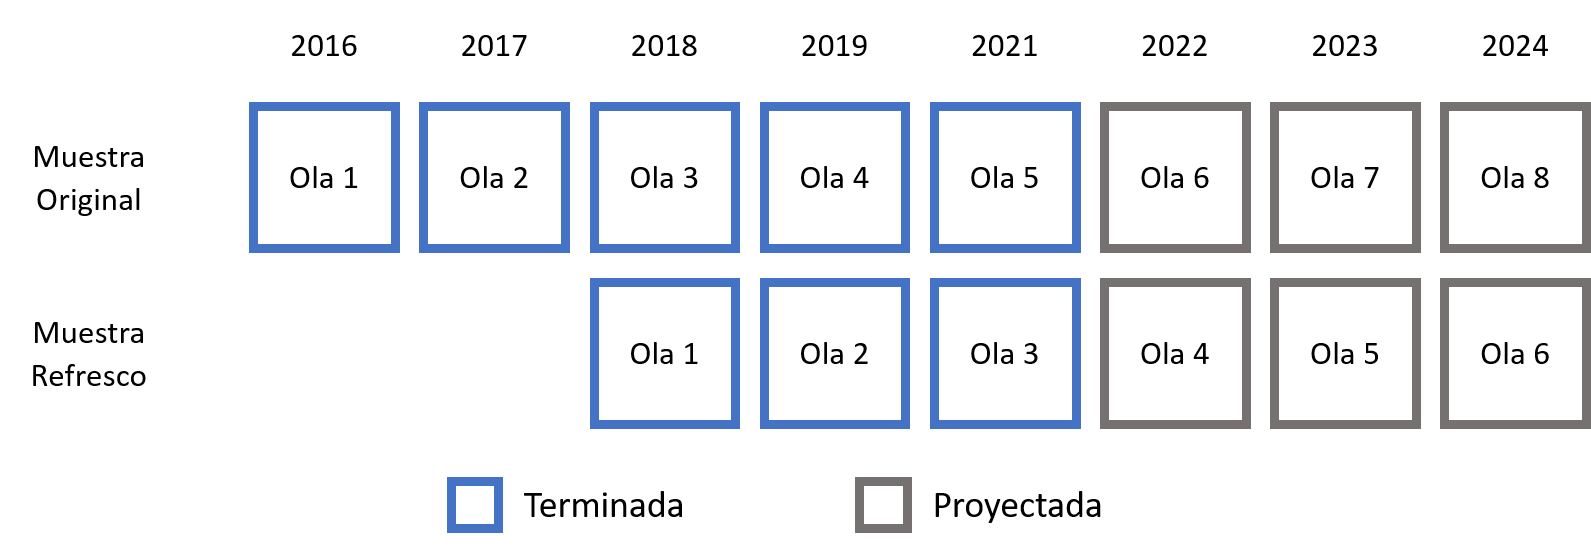
\includegraphics[width=22.1in]{inputs/imagenes/olas_elsoc} 

}

\caption{Mediciones de ELSOC}\label{fig:ilust-olas-elsoc}
\end{figure}

\begin{figure}

{\centering 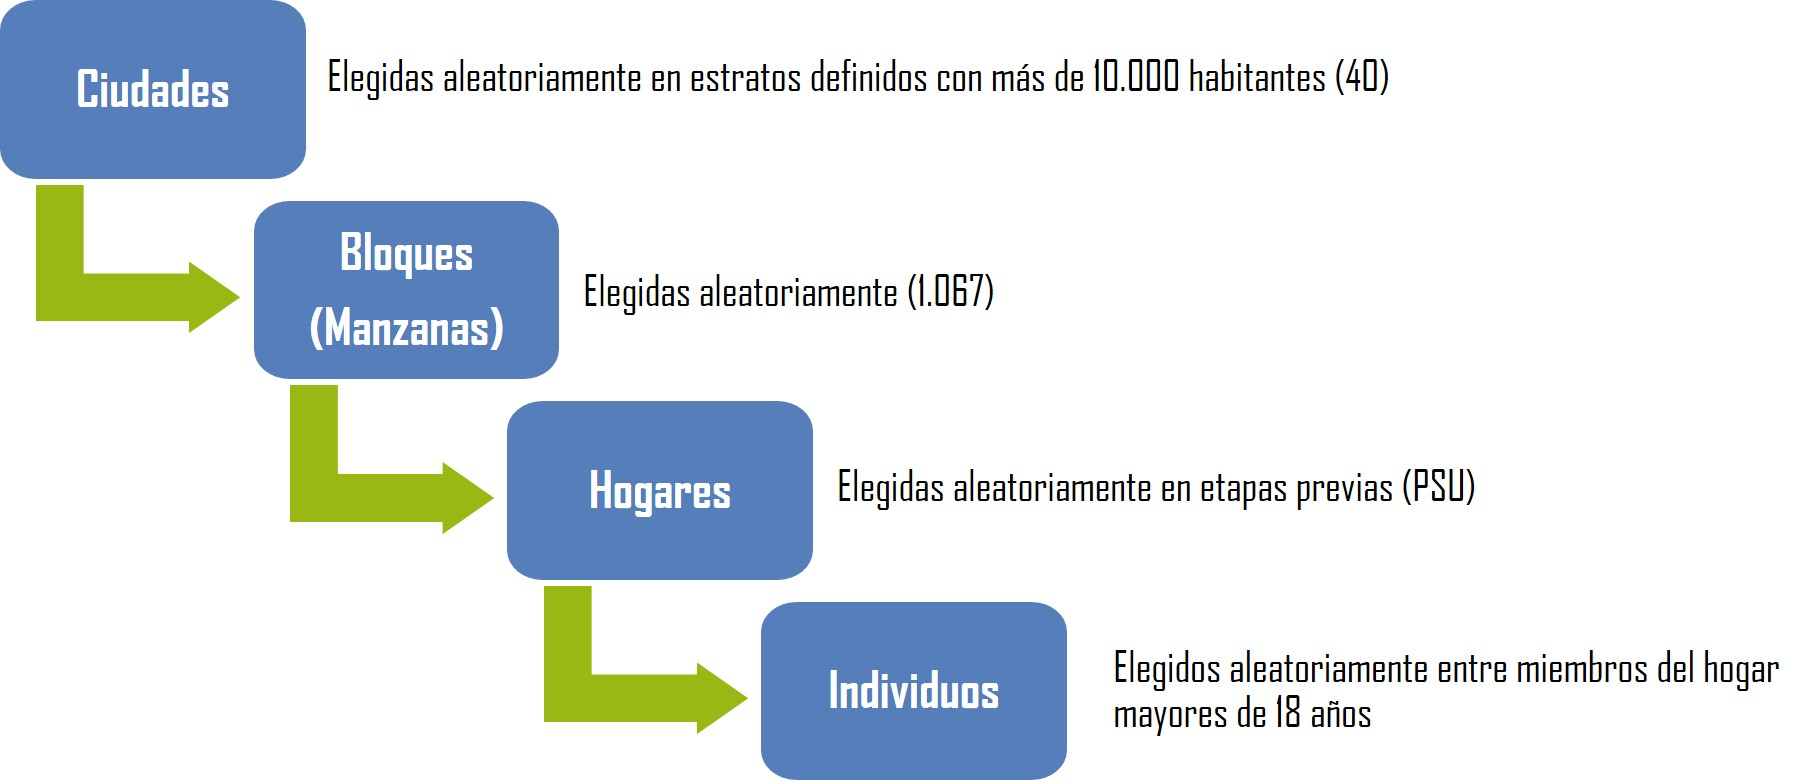
\includegraphics[width=25.24in]{inputs/imagenes/etapas_seleccion} 

}

\caption{Muestreo de ELSOC}\label{fig:ilust-etapas-seleccion}
\end{figure}

\hypertarget{caracteruxedsticas-del-levantamiento-de-datos}{%
\subsection{Características del levantamiento de datos}\label{caracteruxedsticas-del-levantamiento-de-datos}}

\begin{itemize}
\item
  Formato de aplicación: Cuestionario estructurado. Levantamiento en formato CAPI (Encuesta presencial con asistencia de tablet). Excepcionalmente se cambió a formato CATI (Encuesta telefónica con asistencia de tablet) durante 2021, debido a contingencia COVID-19
\item
  Período de Aplicación: entre Julio y Noviembre de cada año. Debido al estallido social, la cuarta medición se aplicó entre el 21 de noviembre de 2019 y el 9 de marzo de 2020. Debido a la pandemia, la quinta medición se aplicó entre el 29 de enero de 2021 y 12 de julio de 2021
\item
  Instrumento: Cuestionario compuesto por preguntas cerradas de carácter simple y múltiple junto a algunas preguntas abiertas. Combina módulos de preguntas permanentes (medidas en todas las olas) y otras intercaladas entre olas
\item
  Cobertura Temática: Contiene siete módulos temáticos: Territorio, Redes y actitudes sociales, Ciudadanía y democracia, Desigualdad y legitimidad, Conflicto social, Salud y bienestar y Caracterización sociodemográfica
\item
  Incentivos a la participación: Entrega de incentivos monetarios para el encuestado (\$ 6.000 CLP) y de material sobre el estudio (ELSOC y COES). Acciones de seguimiento basadas en la información de contacto (correo electrónico para cumpleaños y días festivos)
\item
  Entrenamiento de entrevistadores: Contratación de entrevistadores con experiencia en encuestas complejas y/o longitudinales. Capacitación centralizada y presencial para coordinadores de campo y un subconjunto de entrevistadores en Santiago (incluidos ejercicios prácticos para la implementación del cuestionario, uso de tabletas y protocolo de contacto). Actividades adicionales en otras regiones de Chile. Diseño de un Manual de entrevistador especializado para el proyecto
\item
  Operaciones de Control y Supervisión: Coordinadores de campo supervisan el trabajo de entrevistadores, verificando el número de visitas, el contacto, la identidad del participante y preguntas claves. Organismo ejecutor realiza una supervisión interna de al menos el 10\% de la muestra (entrevistando nuevamente a algunos encuestados), verificando la duración y la respuesta de los participantes
\end{itemize}

\textbf{Organismo Ejecutor}: Levantamiento a cargo de Centro Micro Datos (CMD) de la Universidad de Chile

\hypertarget{atriciuxf3n-de-la-muestra}{%
\section{Atrición de la muestra}\label{atriciuxf3n-de-la-muestra}}

El diseño de ELSOC contempló entrevistar a 3.000 personas en su muestra original y 1.500 en la muestra refresco. Sin embargo, es habitual que en encuestas panel se reduce el número de participantes, dado que algunos optan voluntariamente por dejar de participar y otras personas no pueden ser recontactadas. Este fenómeno es conocido como atrición, y pueden tener efectos nocivos sobre la utilidad de los datos longitudinales. En el caso de ELSOC, la tasa de atrición es comparativamente baja en comparación a otros estudios similares, por lo que no se considera al momento un problema significativo. A pesar de esto, el año 2018 se introduce una muestra refresco para contraarrestar el efecto de la atrición.

El año 2021, la atrición presenta un alza importante debido a la mayor dificultad que implica el levantamiento durante la pandemia de COVID-19 y al cambio de modalidad.

\begin{table}

\caption{\label{tab:tabla-atricion}Atrición de las muestras de ELSOC entre olas}
\centering
\begin{tabular}[t]{c|c|c|c|c}
\hline
\multicolumn{1}{c|}{ } & \multicolumn{2}{c|}{Muestra original} & \multicolumn{2}{c}{Muestra refresco} \\
\cline{2-3} \cline{4-5}
Medición & Muestra lograda & Atrición & Muestra lograda & Atrición\\
\hline
2016 & 2 927 &  &  & \\
\hline
2017 & 2 473 & 15.5\% &  & \\
\hline
2018 & 2 229 & 9.9\% & 1 519 & \\
\hline
2019 & 2 153 & 3.4\% & 1 264 & 16.8\%\\
\hline
2021 & 1 739 & 19.2\% & 1 001 & 20.8\%\\
\hline
\end{tabular}
\end{table}

\hypertarget{atriciuxf3n-acumulada-seguxfan-sexo-grupo-etuxe1reo-nivel-educacional-y-estrato}{%
\subsection{Atrición acumulada según Sexo, Grupo etáreo, Nivel educacional y Estrato}\label{atriciuxf3n-acumulada-seguxfan-sexo-grupo-etuxe1reo-nivel-educacional-y-estrato}}

Para el cálculo de atrición acumulada se considera el período 2016-2021 para la muestra original, y el período 2018-2021 para la muestra refresco

\begin{itemize}
\tightlist
\item
  Según sexo:
\end{itemize}

\begin{table}

\caption{\label{tab:tabla-atricion-sexo}Atrición acumulada de ELSOC, según sexo}
\centering
\begin{tabular}[t]{l|c|c|c|c}
\hline
\multicolumn{1}{c|}{ } & \multicolumn{2}{c|}{Muestra lograda en 2021} & \multicolumn{2}{c}{Atrición acumulada} \\
\cline{2-3} \cline{4-5}
Sexo & Muestra original & Muestra refresco & Muestra original & Muestra refresco\\
\hline
Hombre & 628 & 376 & 46\% & 38\%\\
\hline
Mujer & 1 111 & 625 & 37\% & 31\%\\
\hline
\end{tabular}
\end{table}

\begin{itemize}
\tightlist
\item
  Según grupo etáreo:
\end{itemize}

\begin{table}

\caption{\label{tab:tabla-atricion-edad}Atrición acumulada de ELSOC, según grupo etáreo}
\centering
\begin{tabular}[t]{l|c|c|c|c}
\hline
\multicolumn{1}{c|}{ } & \multicolumn{2}{c|}{Muestra lograda en 2021} & \multicolumn{2}{c}{Atrición acumulada} \\
\cline{2-3} \cline{4-5}
Grupo etáreo & Muestra original & Muestra refresco & Muestra original & Muestra refresco\\
\hline
18-29 & 142 & 173 & 72\% & 49\%\\
\hline
30-49 & 637 & 396 & 45\% & 32\%\\
\hline
50-64 & 609 & 291 & 27\% & 30\%\\
\hline
65 o más & 351 & 141 & 17\% & 22\%\\
\hline
\end{tabular}
\end{table}

\begin{itemize}
\tightlist
\item
  Según nivel educacional:
\end{itemize}

\begin{table}

\caption{\label{tab:tabla-atricion-educ}Atrición acumulada de ELSOC, según nivel educacional}
\centering
\begin{tabular}[t]{l|c|c|c|c}
\hline
\multicolumn{1}{c|}{ } & \multicolumn{2}{c|}{Muestra lograda en 2021} & \multicolumn{2}{c}{Atrición acumulada} \\
\cline{2-3} \cline{4-5}
Nivel educacional & Muestra original & Muestra refresco & Muestra original & Muestra refresco\\
\hline
Basica & 365 & 176 & 44\% & 38\%\\
\hline
Media & 767 & 406 & 39\% & 36\%\\
\hline
Tecnica & 278 & 170 & 42\% & 33\%\\
\hline
Universitaria & 329 & 249 & 39\% & 28\%\\
\hline
\end{tabular}
\end{table}

\begin{itemize}
\tightlist
\item
  Según estrato:
\end{itemize}

\begin{table}

\caption{\label{tab:tabla-atricion-estrato}Atrición acumulada de ELSOC, según estrato}
\centering
\begin{tabular}[t]{l|c|c|c|c}
\hline
\multicolumn{1}{c|}{ } & \multicolumn{2}{c|}{Muestra lograda en 2021} & \multicolumn{2}{c}{Atrición acumulada} \\
\cline{2-3} \cline{4-5}
Estrato & Muestra original & Muestra refresco & Muestra original & Muestra refresco\\
\hline
Santiago & 409 & 262 & 43\% & 38\%\\
\hline
Valparaíso & 214 & 102 & 43\% & 34\%\\
\hline
Concepción & 256 & 138 & 35\% & 27\%\\
\hline
Ciudades
grandes & 254 & 202 & 38\% & 32\%\\
\hline
Ciudades medianas
o pequeñas & 606 & 297 & 41\% & 35\%\\
\hline
\end{tabular}
\end{table}

\hypertarget{foco-en-el-cambio-longitudinal}{%
\subsection{Foco en el cambio longitudinal}\label{foco-en-el-cambio-longitudinal}}

Radiografía del Cambio Social tiene como objetivo fundamental caracterizar la estabilidad y el cambio en opiniones, actitudes y conductas de los participantes a lo largo del tiempo, enfocándose en distintas dimensiones de la cohesión y conflicto en Chile.

Para el logro de dicho objetivo, el presente reporte se centrará en un subconjunto de participantes del estudio: los 1.513 entrevistados y entrevistadas que participaron en las cinco olas de ELSOC (por lo tanto, todos son parte de la muestra original). Dicha submuestra será la base empírica de los hallazgos expuestos en las siguientes secciones.

A continuación se describe a este grupo de participantes según los mismos atributos sociodemográficos (sexo, edad, educación y zona de residencia).

Los resultados presentados a continuación incorporan el diseño muestral complejo de la encuesta, por lo que incorporan los ponderadores muestrales ajustados a población regional y sexo, según estrato y conglomerado muestral.

\begin{figure}

{\centering 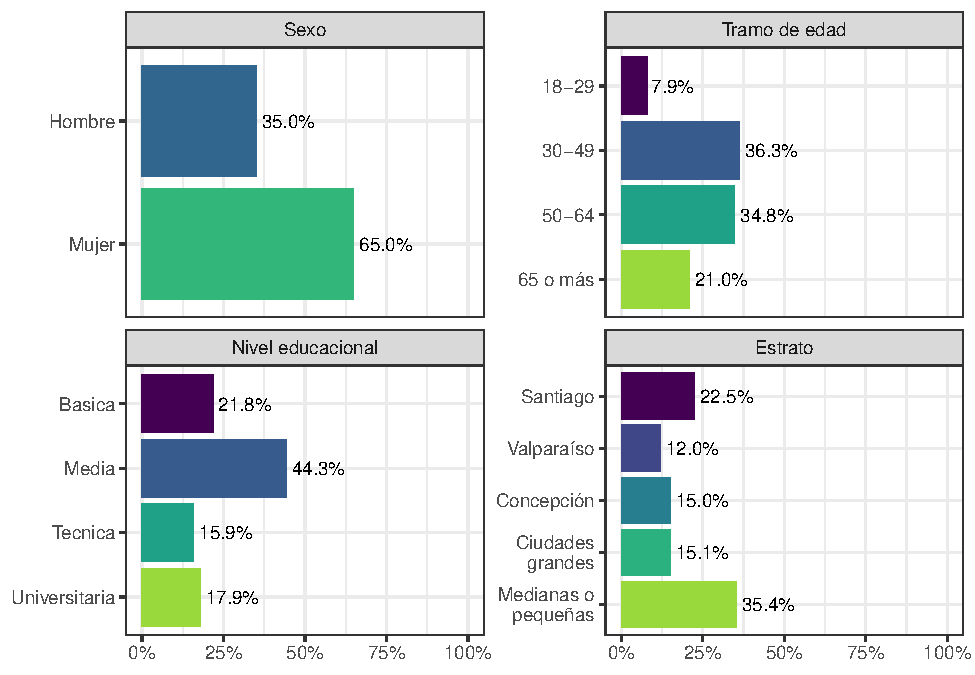
\includegraphics{reporte-elsoc_files/figure-latex/graf-composicion-muestra-1} 

}

\caption{Composición de muestra longitudinal}\label{fig:graf-composicion-muestra}
\end{figure}

\hypertarget{temas-poluxedticos}{%
\chapter{Temas políticos}\label{temas-poluxedticos}}

¿Cómo ha cambiado la sociedad en temas políticos?

\hypertarget{identificaciuxf3n-poluxedtica}{%
\section{Identificación política}\label{identificaciuxf3n-poluxedtica}}

\hypertarget{cuxf3mo-se-posicionan-poluxedticamente-los-chilenos}{%
\subsection{¿Cómo se posicionan políticamente los chilenos?}\label{cuxf3mo-se-posicionan-poluxedticamente-los-chilenos}}

\begin{figure}

{\centering 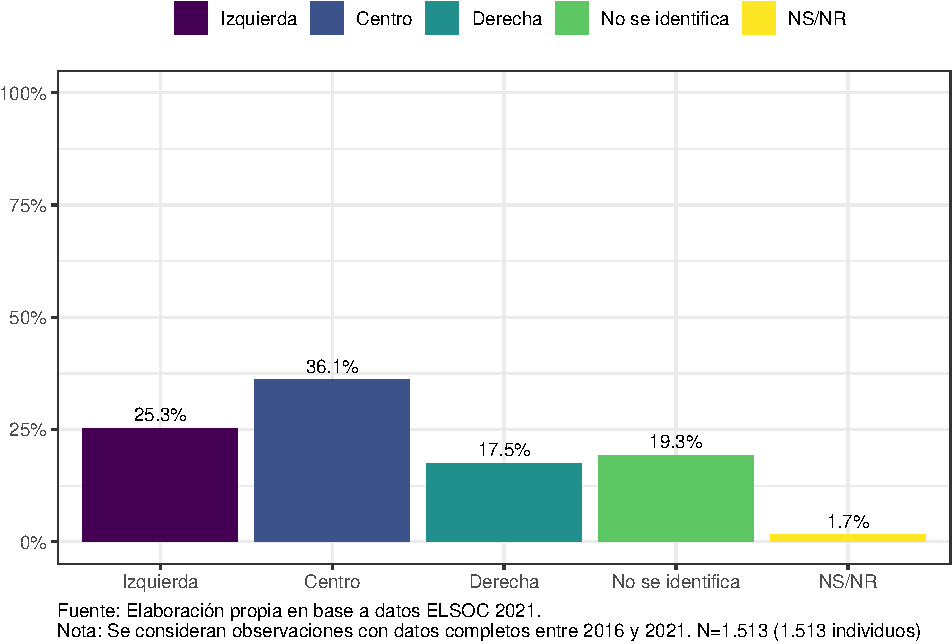
\includegraphics{reporte-elsoc_files/figure-latex/graf-idpolitica-1} 

}

\caption{Identificación política (2021)}\label{fig:graf-idpolitica}
\end{figure}

Entre 2016 y 2021 la identificación con la izquierda se ha mantenido estable (25,3\% en 2021), mientras que
el centro y la derecha han aumentado su participación (de 24,8\% en 2016 a 36,1\% en 2021, y de 14,1\% a 17,5\%, respectivament), en desmedro de la no identifiación política, que disminuyó de 35,8\% a 19,3\%.

\begin{figure}

{\centering 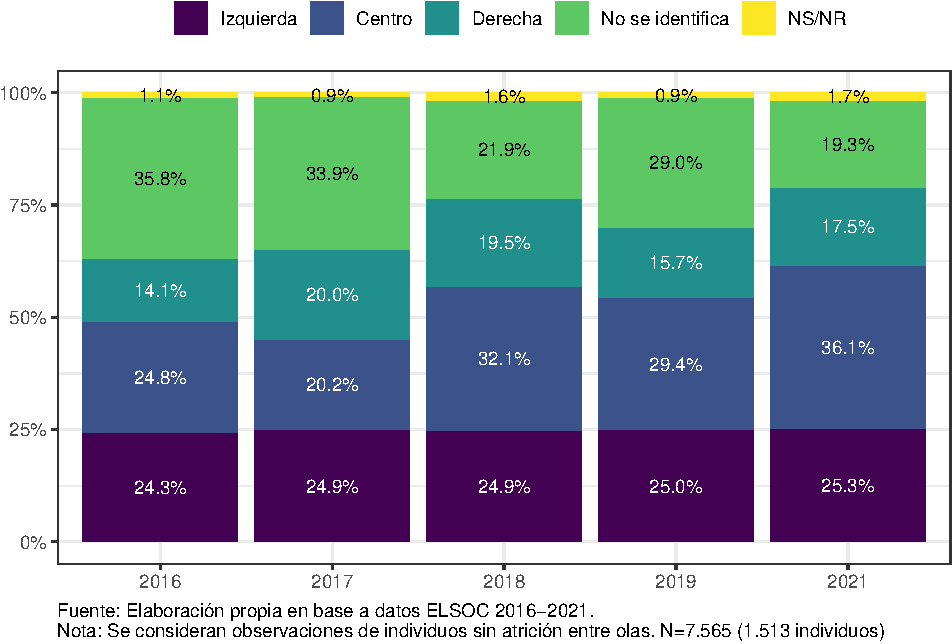
\includegraphics{reporte-elsoc_files/figure-latex/graf-idpolitica-ola-1} 

}

\caption{Identificación política, según ola del estudio}\label{fig:graf-idpolitica-ola}
\end{figure}

Aunque los porcentajes son relativamente estables, esconden una alta fluidez en la identificación con las diferentes posiciones políticas por año.

\begin{figure}

{\centering 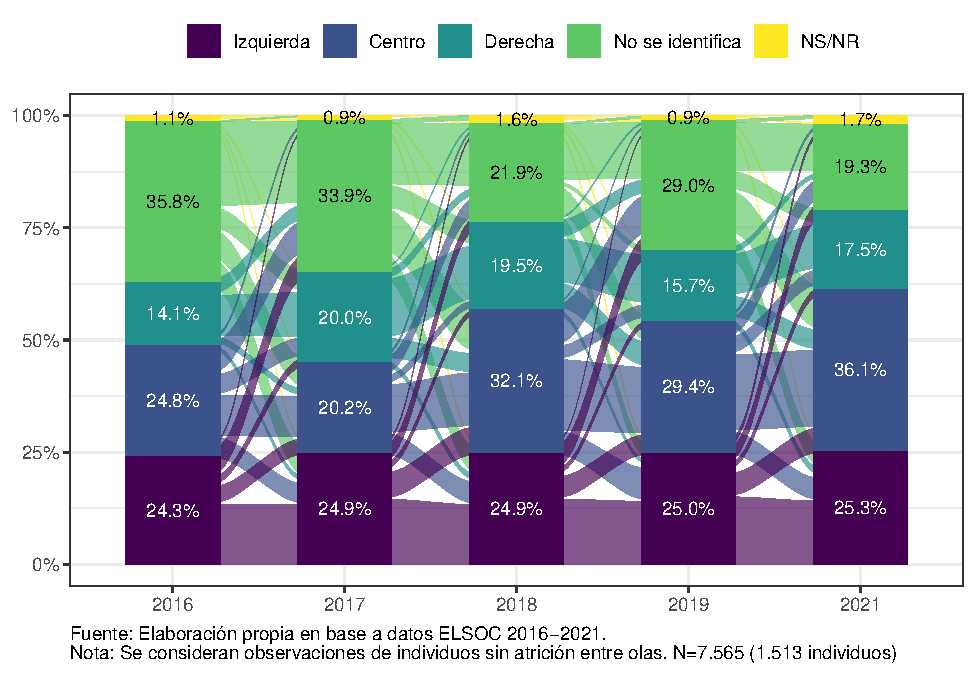
\includegraphics{reporte-elsoc_files/figure-latex/graf-alluvial-idpolitica-ola-1} 

}

\caption{Cambios en la identificación política, según ola del estudio}\label{fig:graf-alluvial-idpolitica-ola}
\end{figure}

De manera consistente aproximadamente 48\% de la población cambia su posición política cada año

\begin{figure}

{\centering 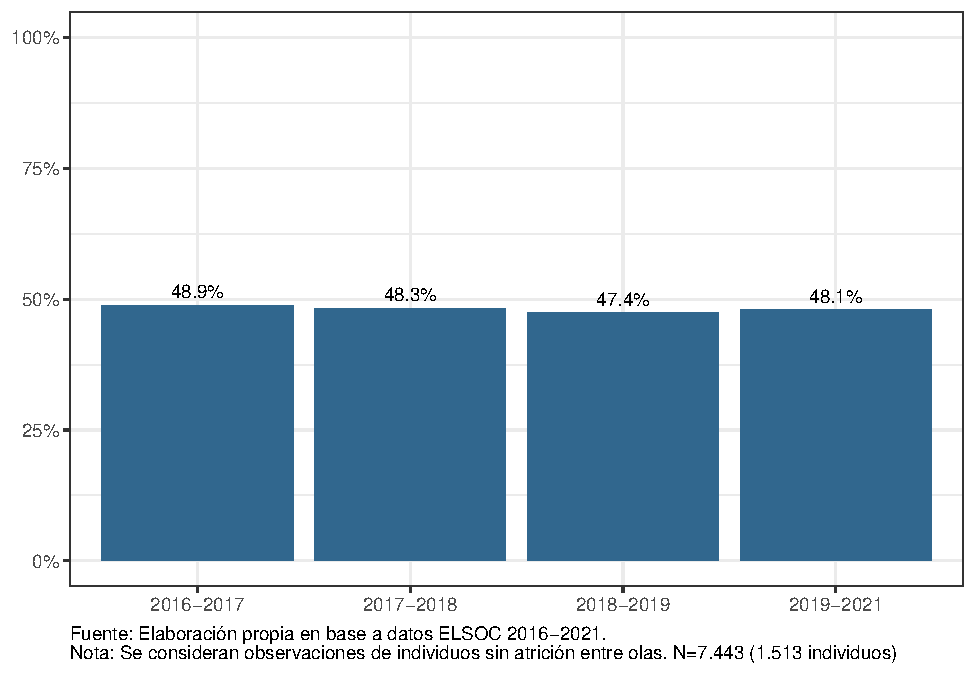
\includegraphics{reporte-elsoc_files/figure-latex/graf-cambios-idpolitica-ola-1} 

}

\caption{Cambios en identificación política, según ola}\label{fig:graf-cambios-idpolitica-ola}
\end{figure}

El grupo político más estable (comparando posiciones politicas entre 2016 y 2021) es el de centro: 54,0\% de quienes se posicionaban políticamente de Centro, lo hicieron también en 2021. En contraste, la No identificación política es la menos estable: solo 31,3\% de quienes no se identificaban políticamente en 2016, lo hicieron también en 2021. Para la izquierda y la derecha, estos porcentajes son 47,8\% y 47,6\%, respectivamente.

\begin{figure}

{\centering 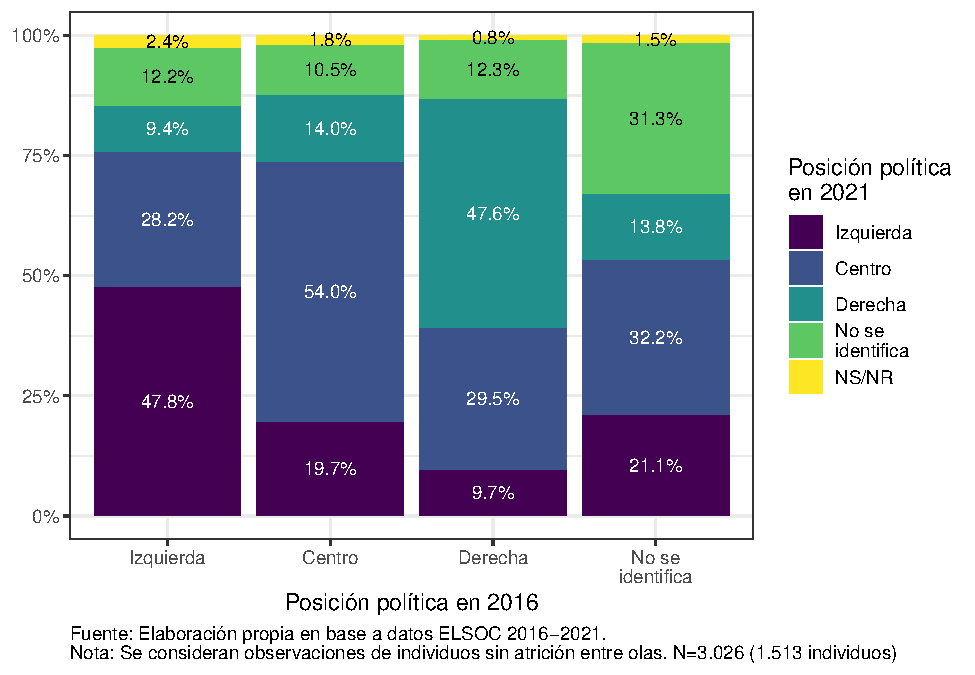
\includegraphics{reporte-elsoc_files/figure-latex/graf-cambios-idpol-idpol-1} 

}

\caption{Cambios en identificación política entre 2016 y 2021}\label{fig:graf-cambios-idpol-idpol}
\end{figure}

A mayor edad mayor estabilidad en la posición política entre años

\begin{figure}

{\centering 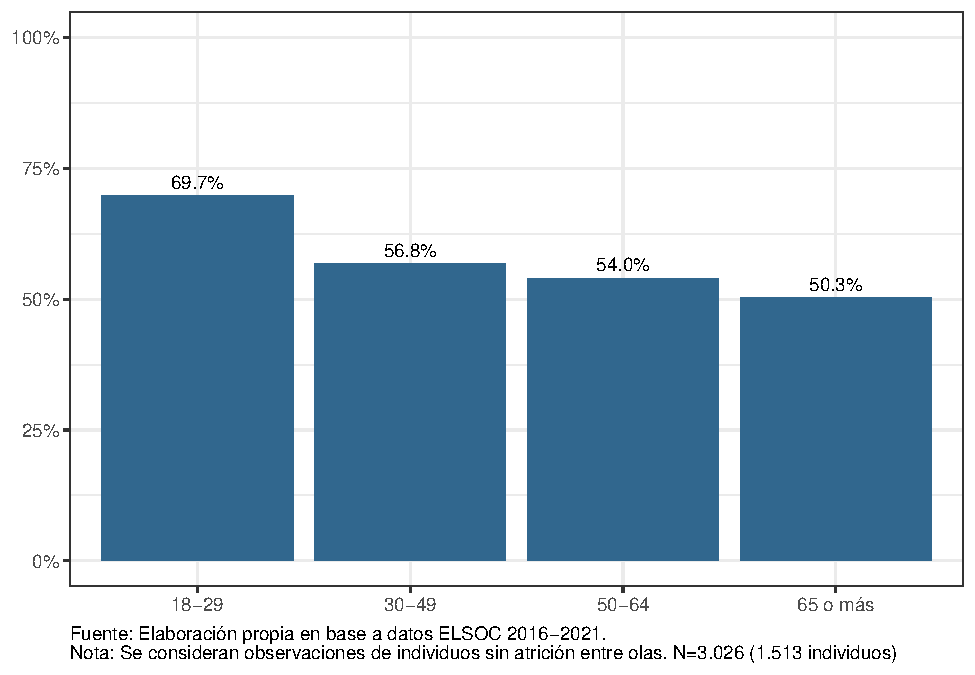
\includegraphics{reporte-elsoc_files/figure-latex/graf-cambios-idpolitica-edad-1} 

}

\caption{Cambios en identificación política, según grupo etáreo}\label{fig:graf-cambios-idpolitica-edad}
\end{figure}

\hypertarget{interuxe9s-en-la-poluxedtica-y-participaciuxf3n-ciudadana}{%
\subsection{Interés en la política y participación ciudadana}\label{interuxe9s-en-la-poluxedtica-y-participaciuxf3n-ciudadana}}

\begin{figure}

{\centering 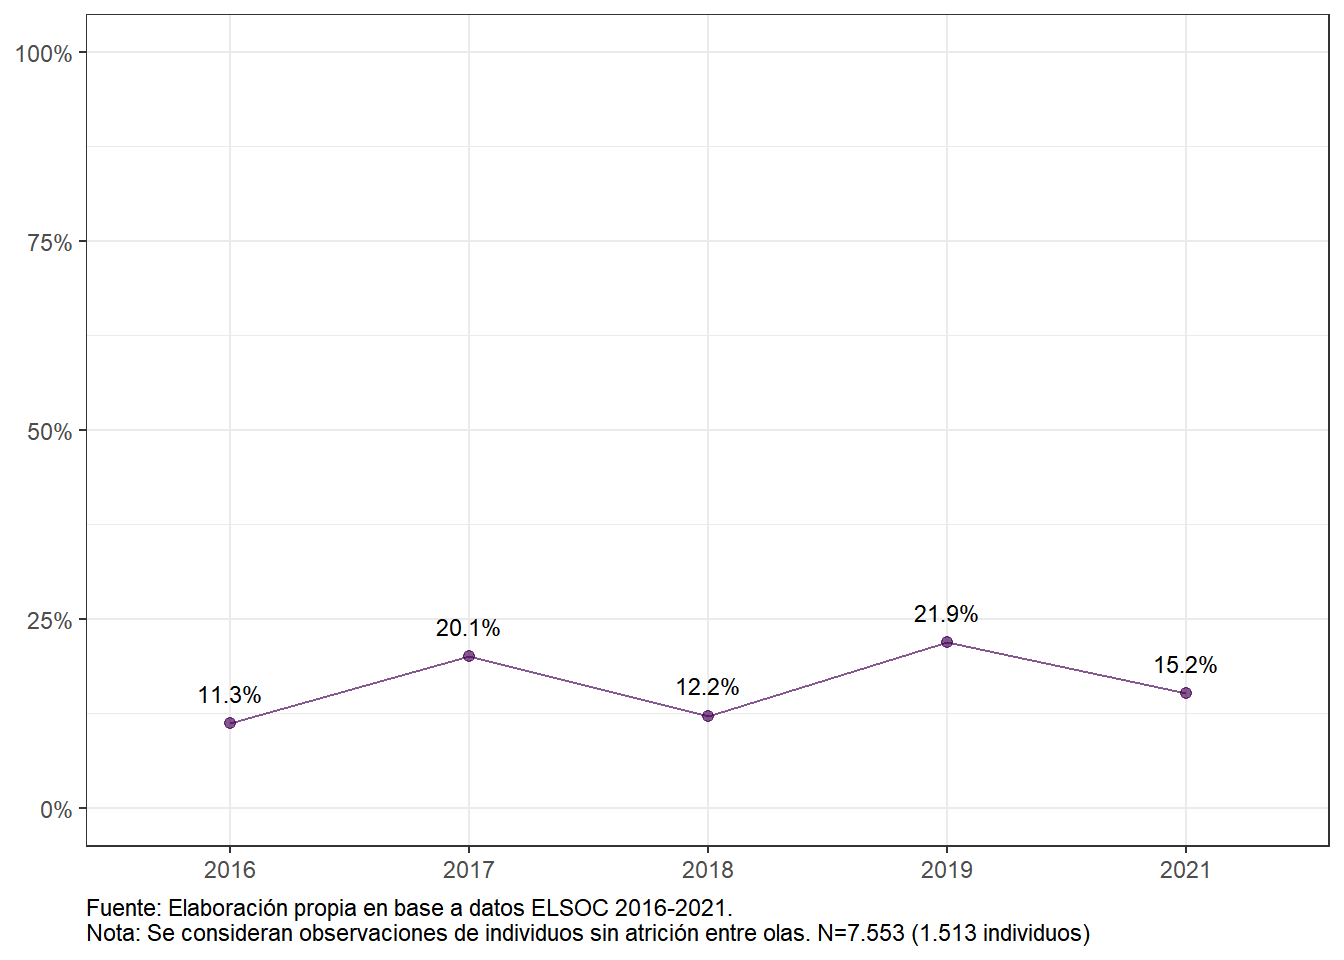
\includegraphics{reporte-elsoc_files/figure-latex/graf-interespolitica-ola-1} 

}

\caption{Interés en política, según ola del estudio}\label{fig:graf-interespolitica-ola}
\end{figure}

\begin{figure}

{\centering 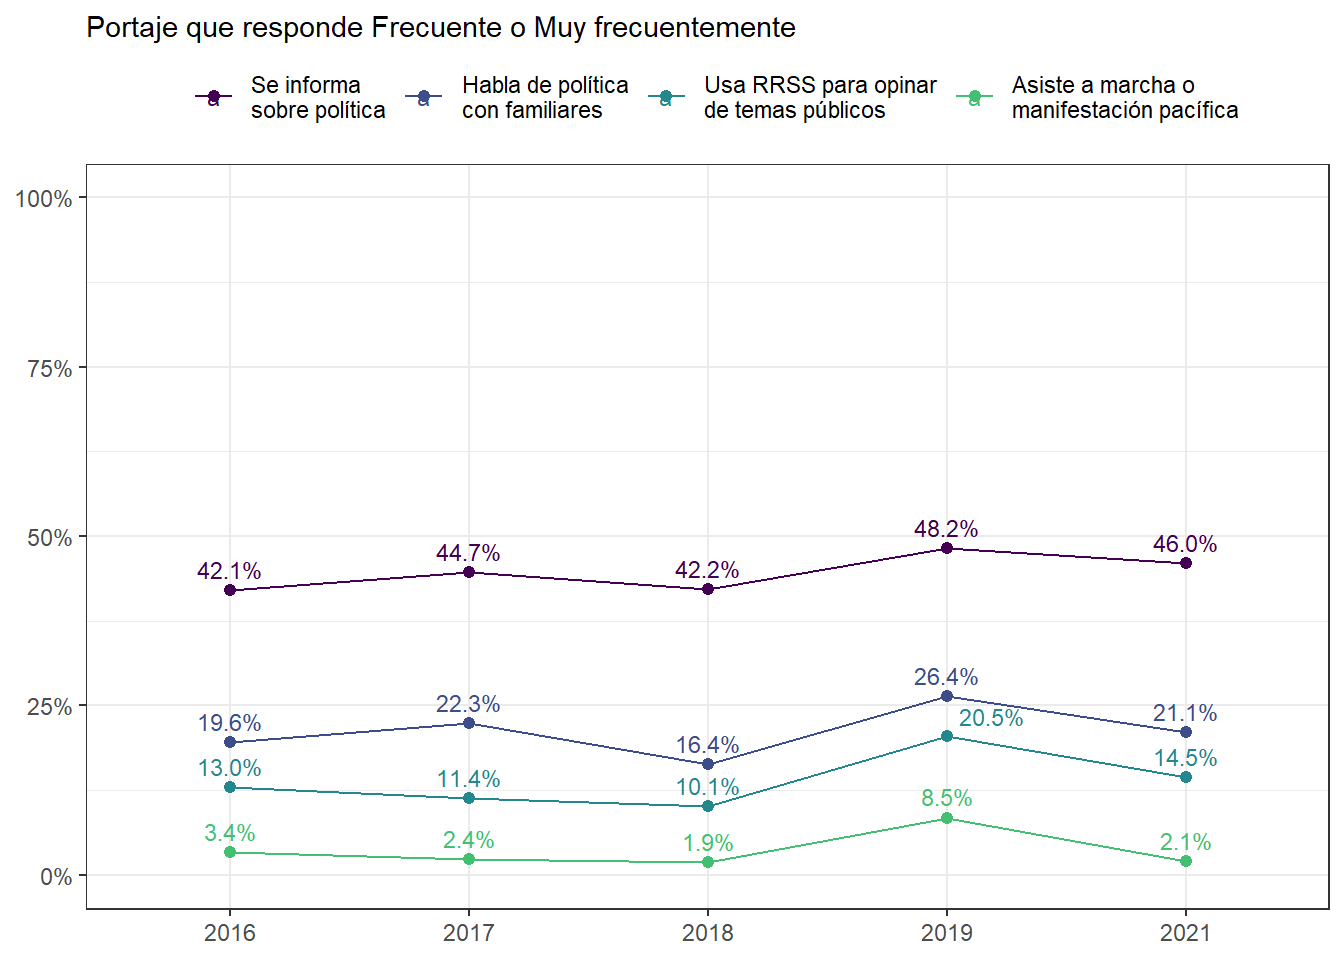
\includegraphics{reporte-elsoc_files/figure-latex/graf-participciudadana-ola-1} 

}

\caption{Participación ciudadana, según ola del estudio}\label{fig:graf-participciudadana-ola}
\end{figure}

\begin{figure}

{\centering 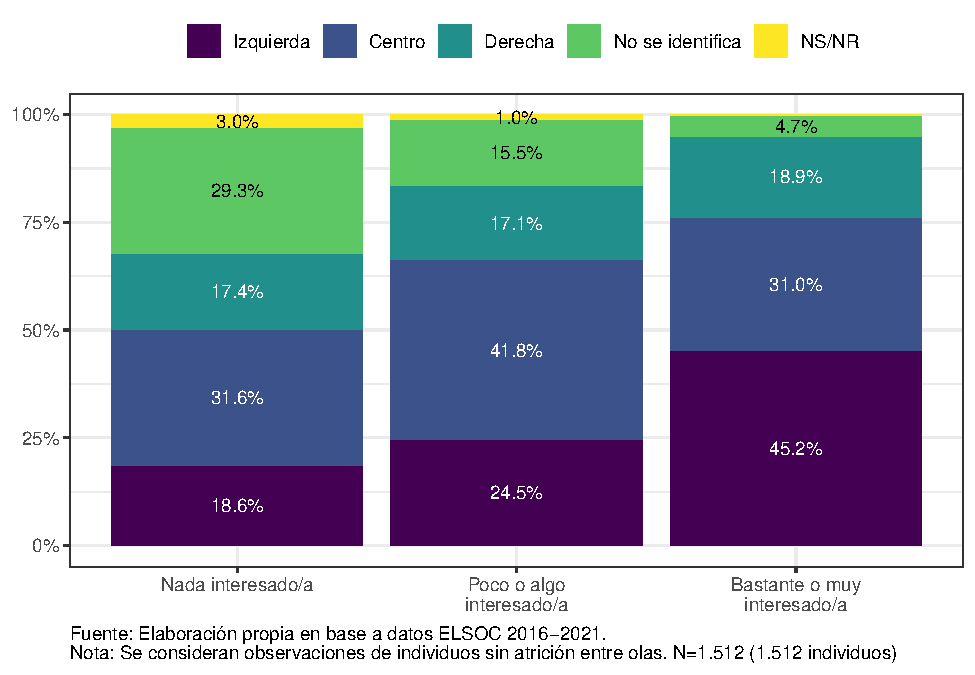
\includegraphics{reporte-elsoc_files/figure-latex/graf-idpolitica-interespolitica-1} 

}

\caption{Identificación política, según grado de interes en la política (2021)}\label{fig:graf-idpolitica-interespolitica}
\end{figure}

\hypertarget{opiniuxf3n-en-temas-de-discusiuxf3n-puxfablica}{%
\subsection{Opinión en temas de discusión pública}\label{opiniuxf3n-en-temas-de-discusiuxf3n-puxfablica}}

\begin{figure}

{\centering 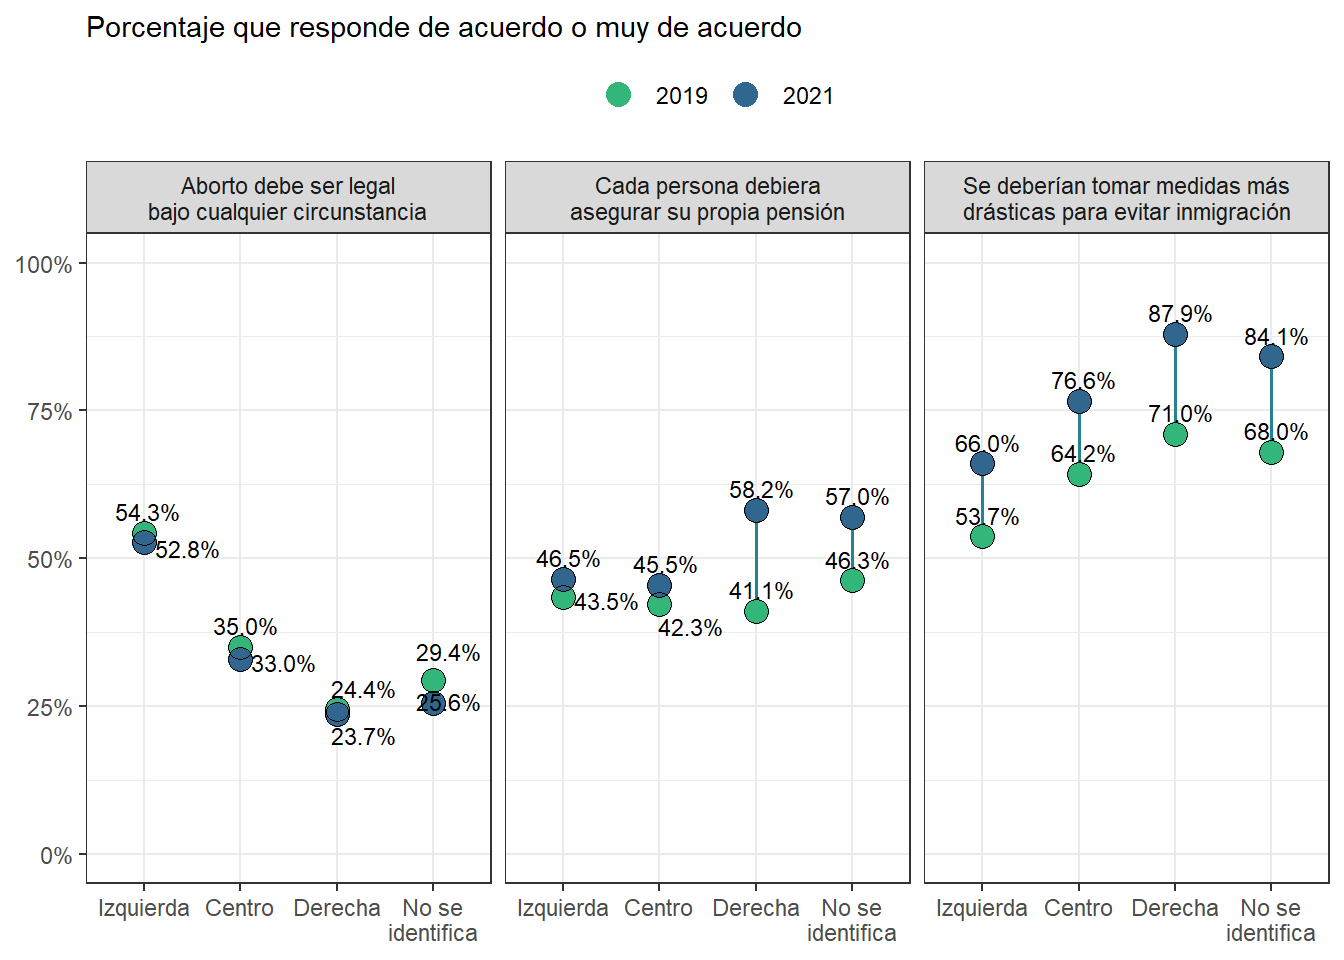
\includegraphics{reporte-elsoc_files/figure-latex/graf-temaspublicos-idpolitica-1} 

}

\caption{Acuerdo con temas de discusión pública, según posición política (2019-2021)}\label{fig:graf-temaspublicos-idpolitica}
\end{figure}

\hypertarget{movimientos-sociales-y-acciones-colectivas}{%
\section{Movimientos Sociales y Acciones Colectivas}\label{movimientos-sociales-y-acciones-colectivas}}

\hypertarget{ciclo-de-movilizaciuxf3n-poluxedtica-y-estallido-social}{%
\subsection{Ciclo de movilización política y estallido social}\label{ciclo-de-movilizaciuxf3n-poluxedtica-y-estallido-social}}

\begin{figure}

{\centering 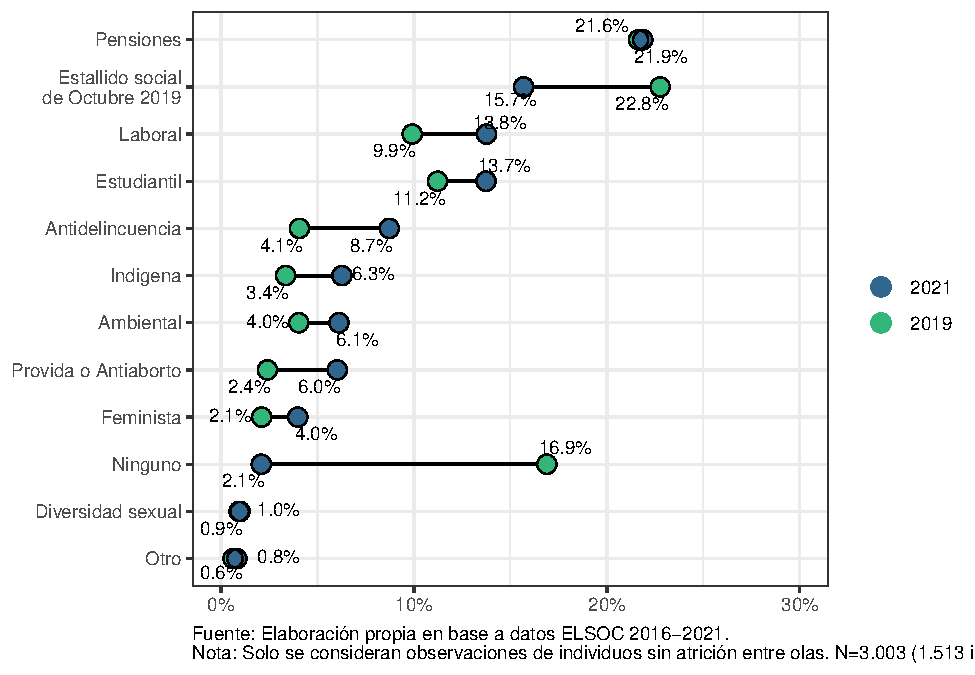
\includegraphics{reporte-elsoc_files/figure-latex/graf-movsocial-1} 

}

\caption{¿Cuál de los siguientes movimientos sociales más valora? (2019-2021)}\label{fig:graf-movsocial}
\end{figure}

Clasificacindo los movimientos sociales en las categorías ``Progresistas'' y ``Conservadores,'' se ve un claro aumento en la valoración de movimientos sociales progresistas.

Los movimientos sociales que se clasifican como progresistas son:

\begin{itemize}
\tightlist
\item
  Movimiento social de apoyo a la causa estudiantil
\item
  Movimiento social de apoyo a demandas laborales
\item
  Movimiento social de grupos ambientalistas
\item
  Movimiento social de apoyo a las demandas indígena
\item
  Movimiento social de apoyo a la diversidad sexual
\item
  Movimiento feminista o de apoyo a la igualdad de género
\item
  Movimiento por el cambio al sistema de pensiones
\item
  Estallido social del 18 de Octubre de 2019
\end{itemize}

Mientras que los Conservadores:

\begin{itemize}
\tightlist
\item
  Movimiento social provida o antiaborto
\item
  Movimiento social antidelincuencia
\end{itemize}

\begin{figure}

{\centering 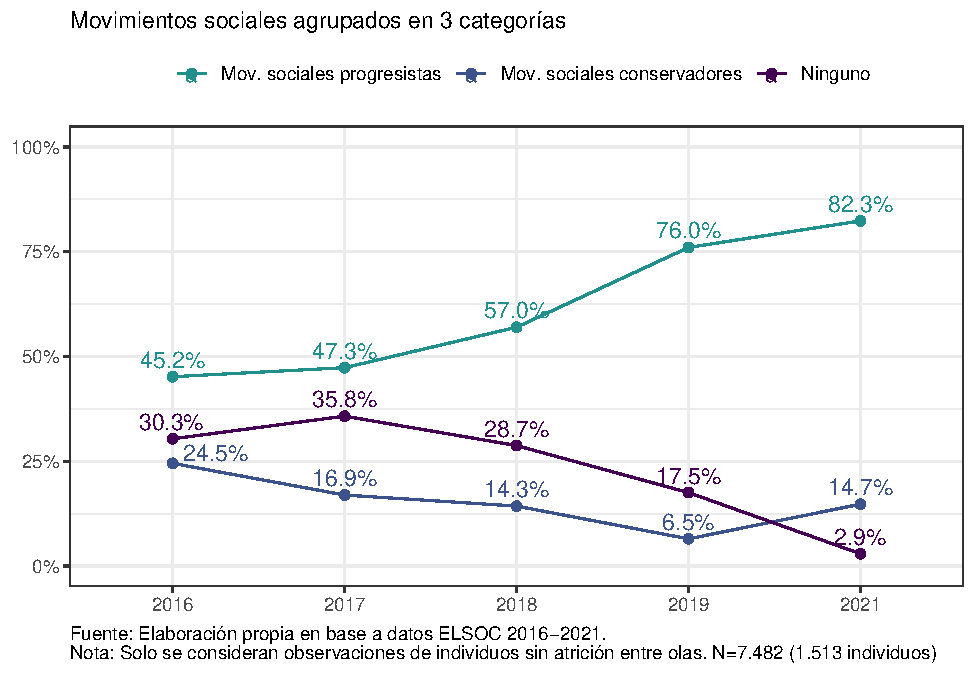
\includegraphics{reporte-elsoc_files/figure-latex/graf-movsociales-movsocial-olas-1} 

}

\caption{Movimiento social que más valora, Según ola}\label{fig:graf-movsociales-movsocial-olas}
\end{figure}

\textbackslash begin\{figure\}

\{\centering 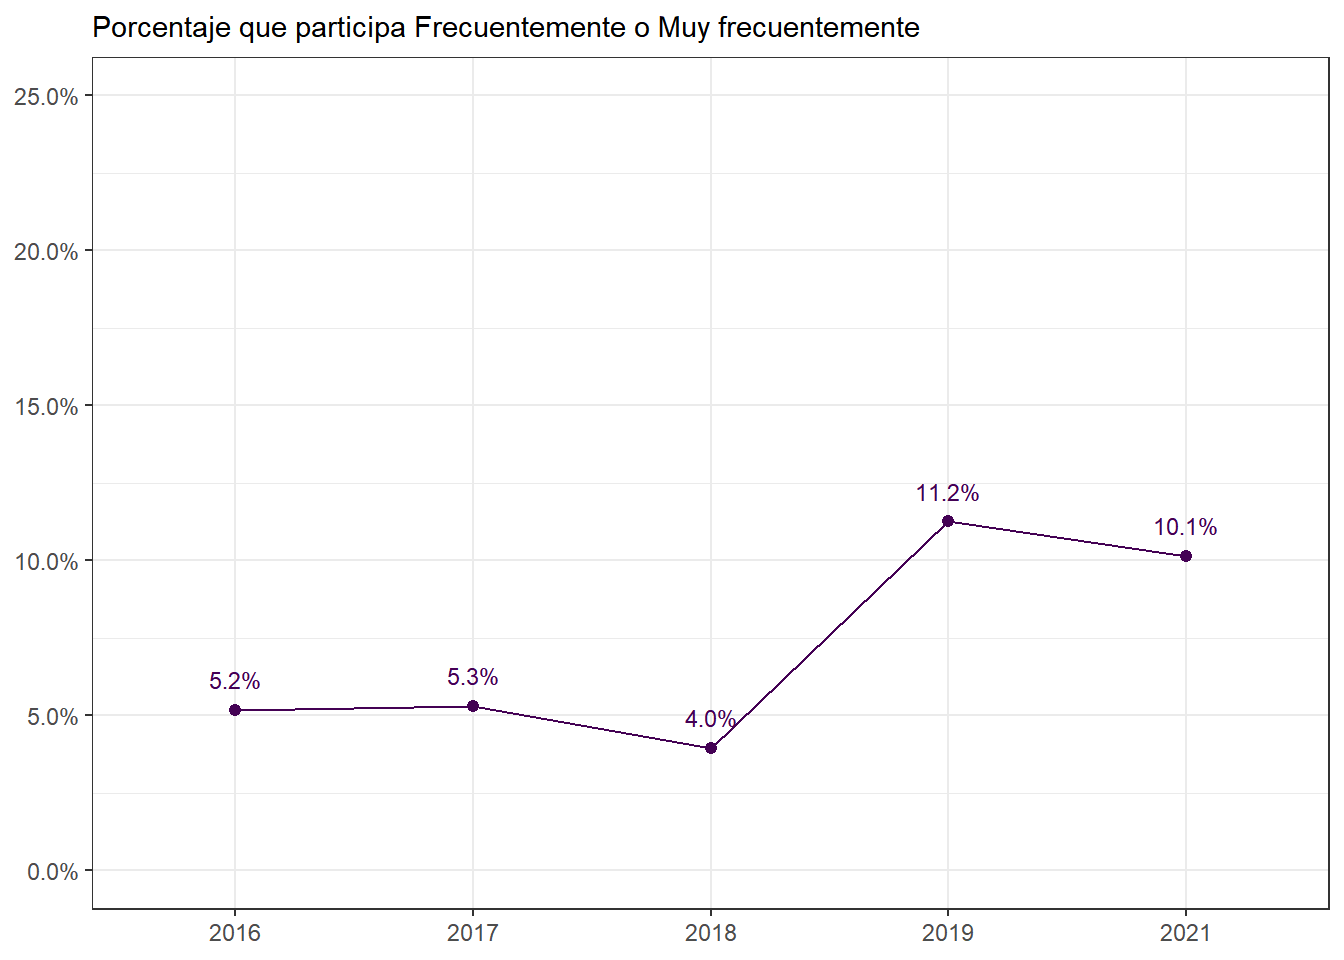
\includegraphics{reporte-elsoc_files/figure-latex/graf-particip_movsocial-olas-1}

\}

\caption{Participación en movimientos sociales valorados, según ola}

(\#fig:graf-particip\_movsocial-olas)
\textbackslash end\{figure\}

\textbackslash begin\{figure\}

\{\centering 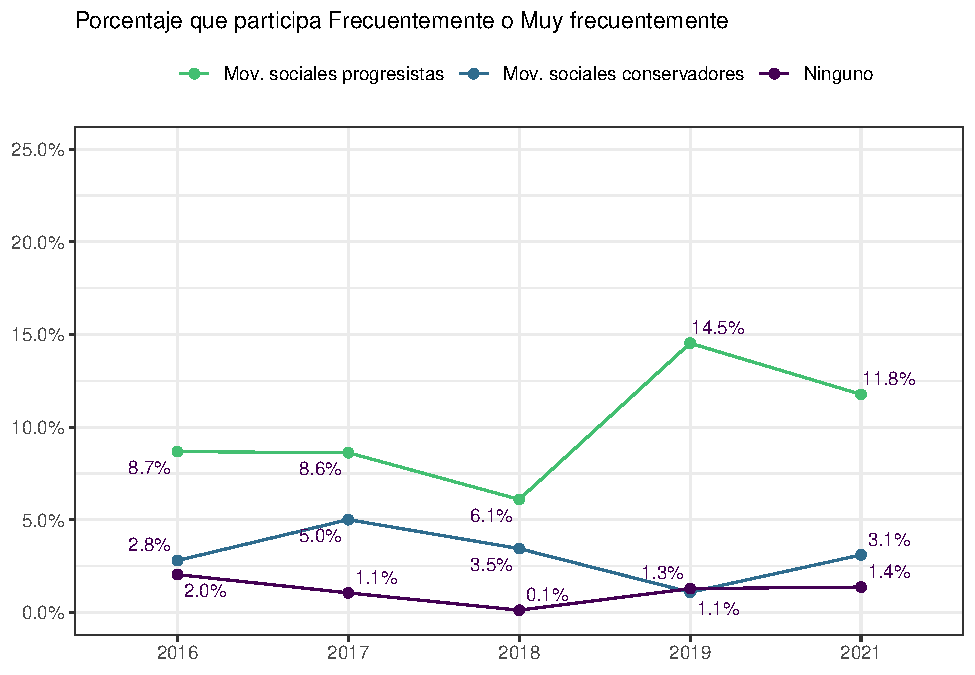
\includegraphics{reporte-elsoc_files/figure-latex/graf-particip_movsociales2-ola-1}

\}

\caption{Participación en movimientos sociales valorados, según ola}

(\#fig:graf-particip\_movsociales2-ola)
\textbackslash end\{figure\}

\hypertarget{justificaciuxf3n-de-la-violencia}{%
\section{Justificación de la Violencia}\label{justificaciuxf3n-de-la-violencia}}

\hypertarget{justificaciuxf3n-de-la-violencia-para-el-control-social}{%
\subsection{Justificación de la violencia para el control social}\label{justificaciuxf3n-de-la-violencia-para-el-control-social}}

\textbackslash begin\{figure\}

\{\centering 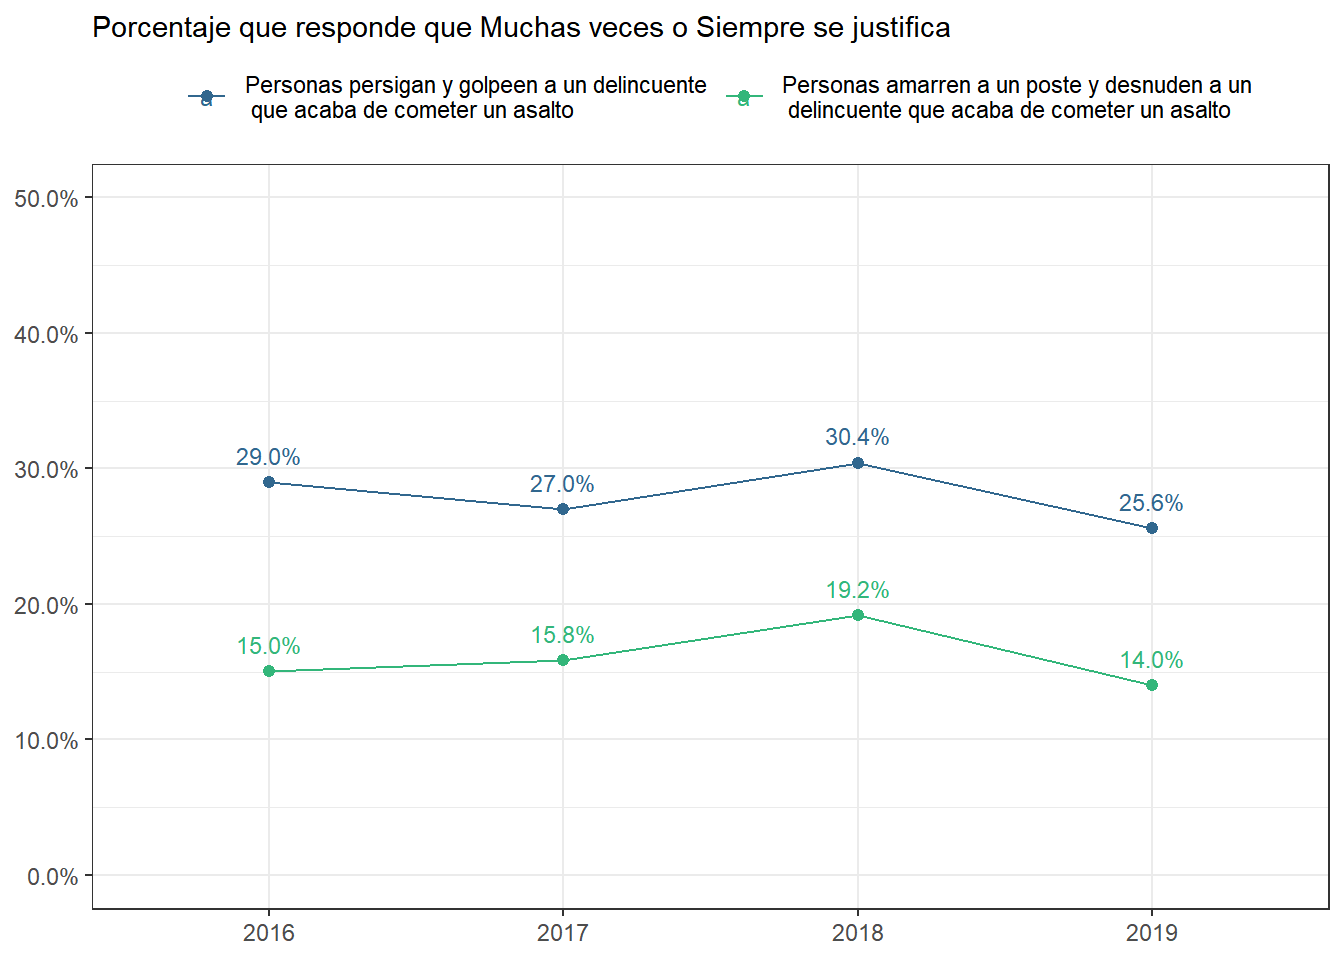
\includegraphics{reporte-elsoc_files/figure-latex/graf-just_violencia1-ola-1}

\}

\caption{Justificación de la violencia a manos de ciudadanos, según ola}

(\#fig:graf-just\_violencia1-ola)
\textbackslash end\{figure\}

\textbackslash begin\{figure\}

\{\centering 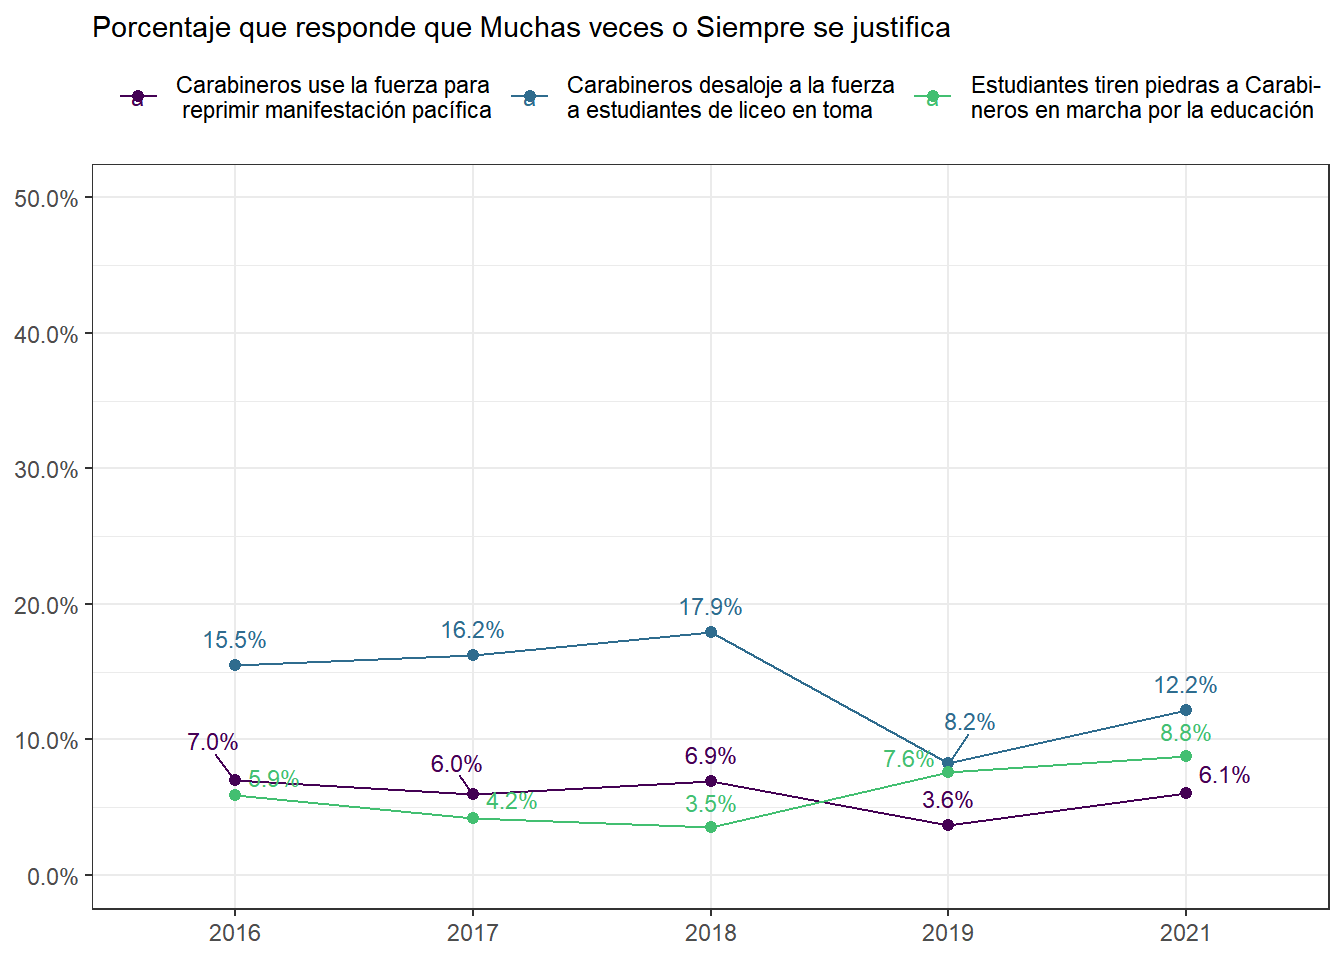
\includegraphics{reporte-elsoc_files/figure-latex/graf-just_violencia2-ola-1}

\}

\caption{Justificación de la violencia, según ola}

(\#fig:graf-just\_violencia2-ola)
\textbackslash end\{figure\}

\hypertarget{confianza-interpersonal-y-en-instituciones}{%
\section{Confianza interpersonal y en instituciones}\label{confianza-interpersonal-y-en-instituciones}}

\hypertarget{confianza-interpersonal}{%
\subsection{Confianza interpersonal}\label{confianza-interpersonal}}

\textbackslash begin\{figure\}

\{\centering 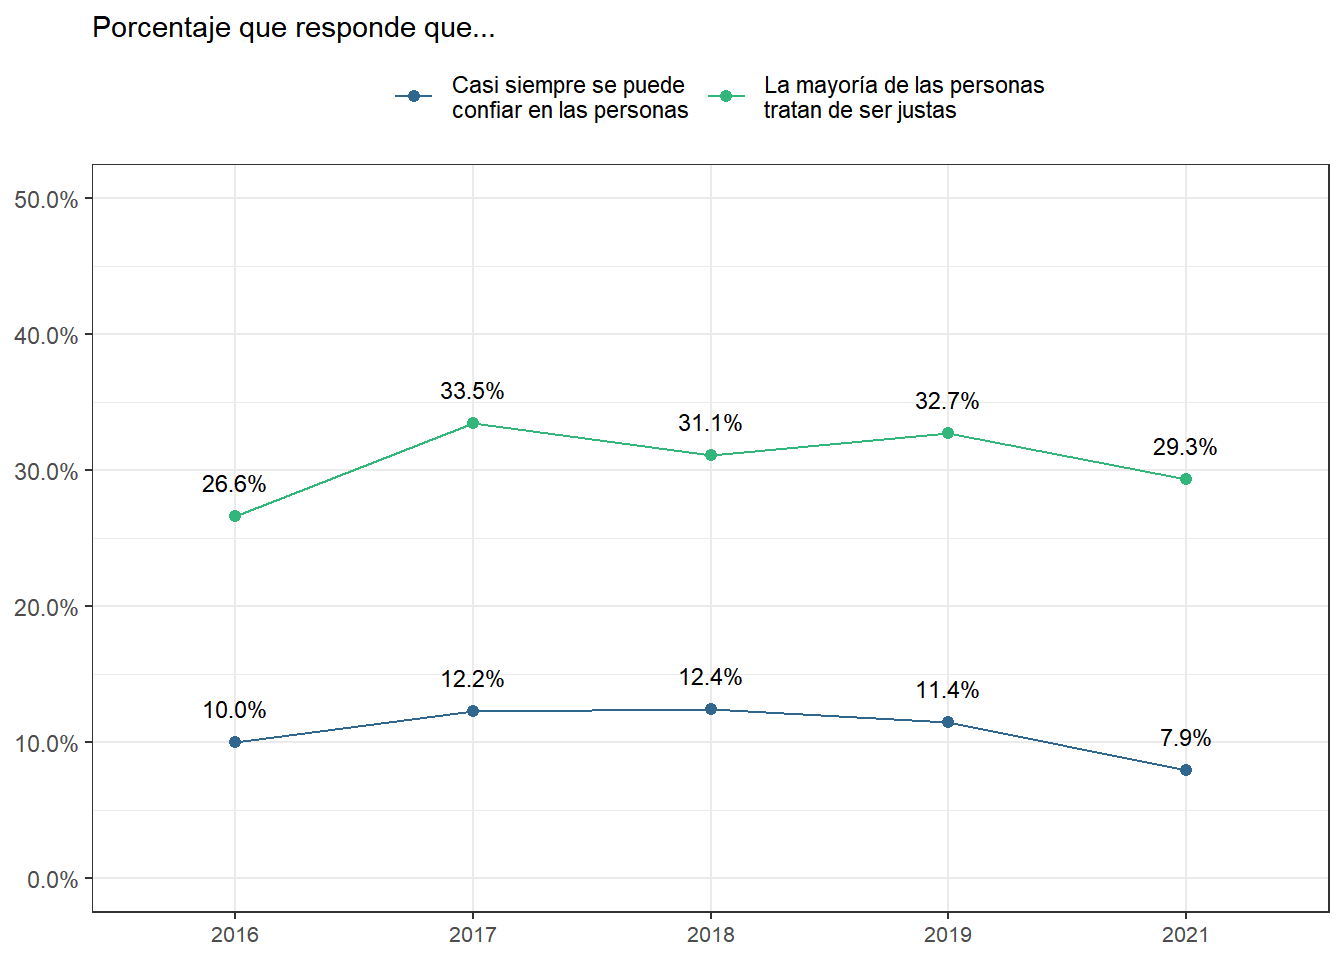
\includegraphics{reporte-elsoc_files/figure-latex/graf-confianza_interpersonal-ola-1}

\}

\caption{Confianza interpersonal, según ola}

(\#fig:graf-confianza\_interpersonal-ola)
\textbackslash end\{figure\}

\textbackslash begin\{figure\}

\{\centering 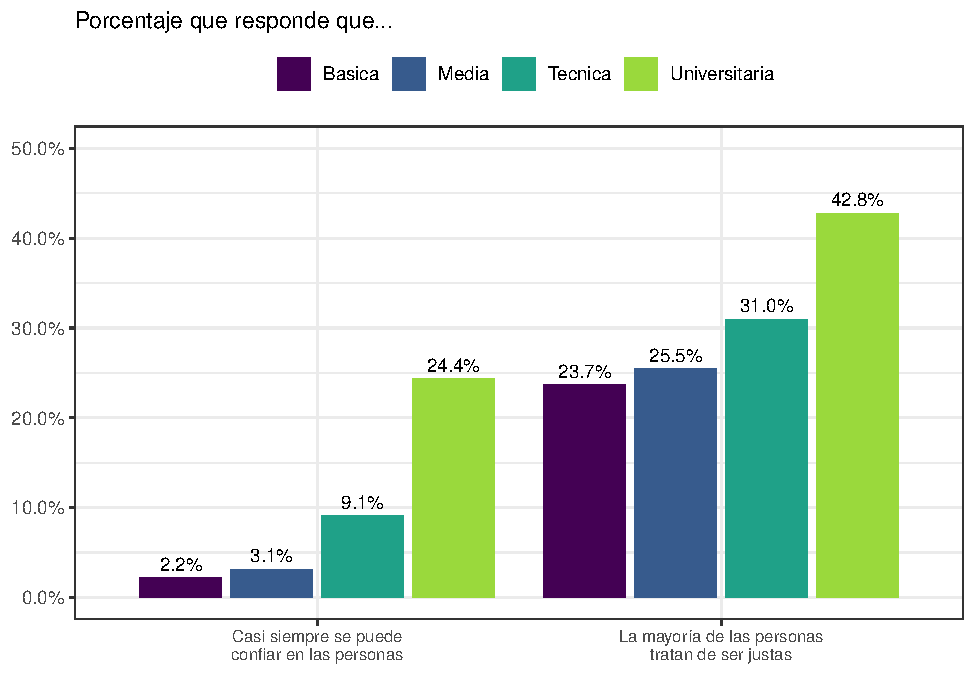
\includegraphics{reporte-elsoc_files/figure-latex/graf-confianza_interpersonal-educ-1}

\}

\caption{Confianza interpersonal (2021), según nivel educacional}

(\#fig:graf-confianza\_interpersonal-educ)
\textbackslash end\{figure\}

\textbackslash begin\{figure\}

\{\centering 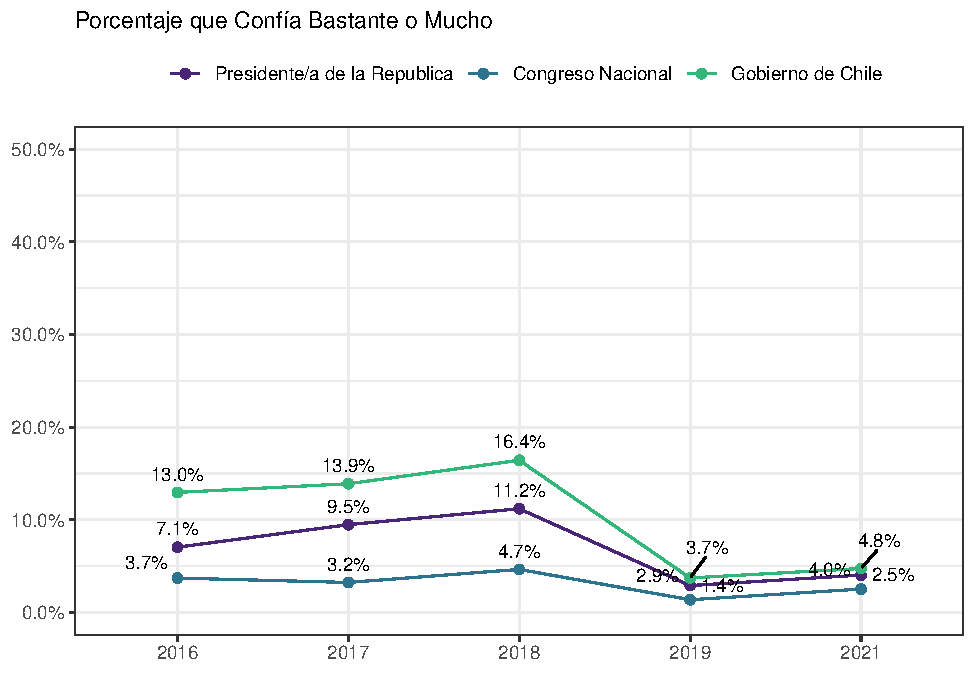
\includegraphics{reporte-elsoc_files/figure-latex/graf-conf_instituciones1-ola-1}

\}

\caption{Grado de confianza en instituciones, según ola}

(\#fig:graf-conf\_instituciones1-ola)
\textbackslash end\{figure\}

\textbackslash begin\{figure\}

\{\centering 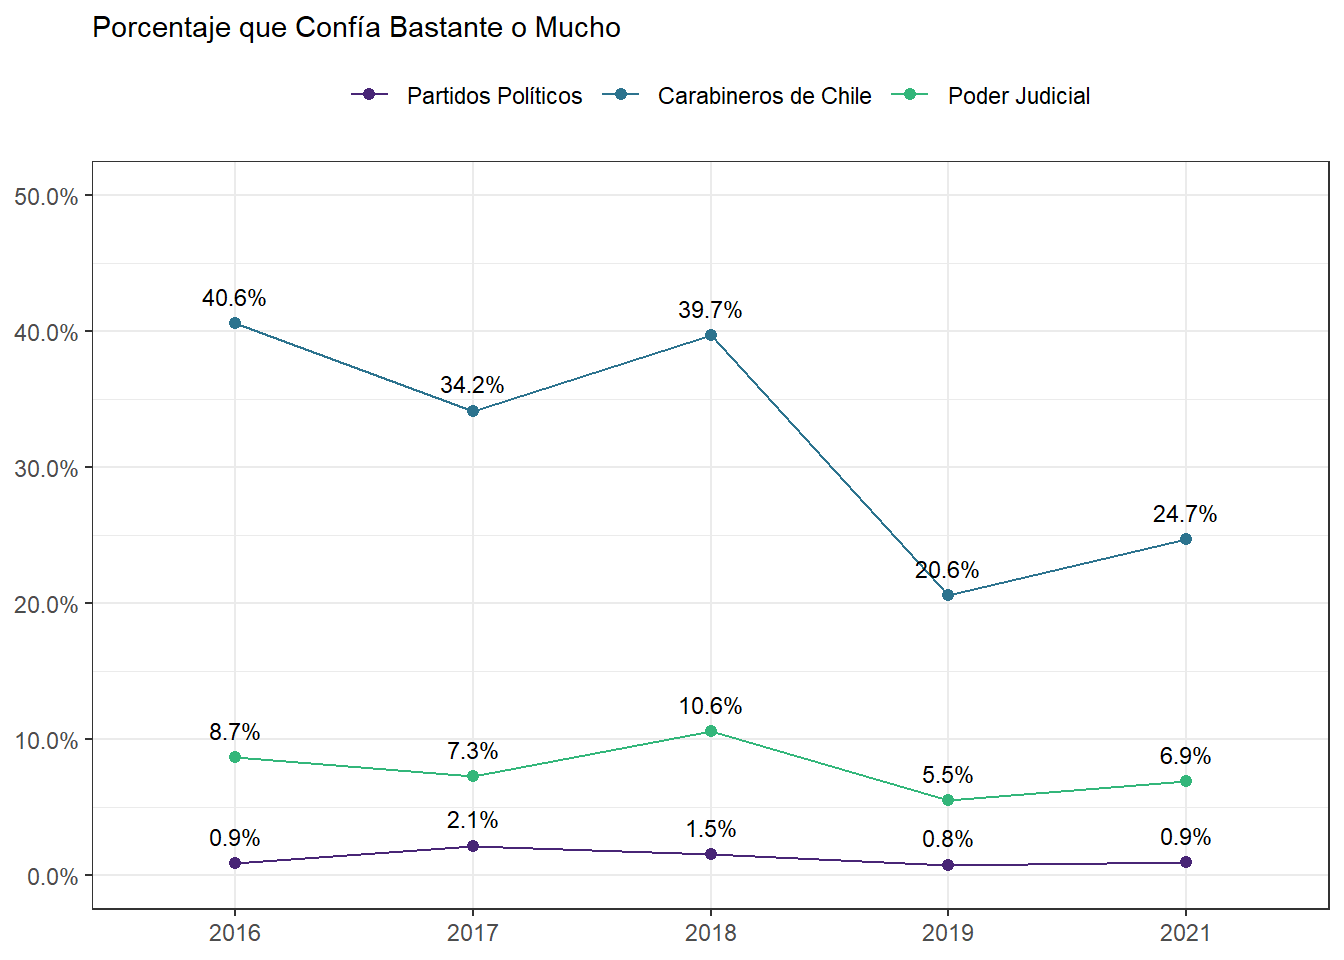
\includegraphics{reporte-elsoc_files/figure-latex/graf-conf_instituciones2-ola-1}

\}

\caption{Grado de confianza en instituciones, según ola}

(\#fig:graf-conf\_instituciones2-ola)
\textbackslash end\{figure\}

\textbackslash begin\{figure\}

\{\centering 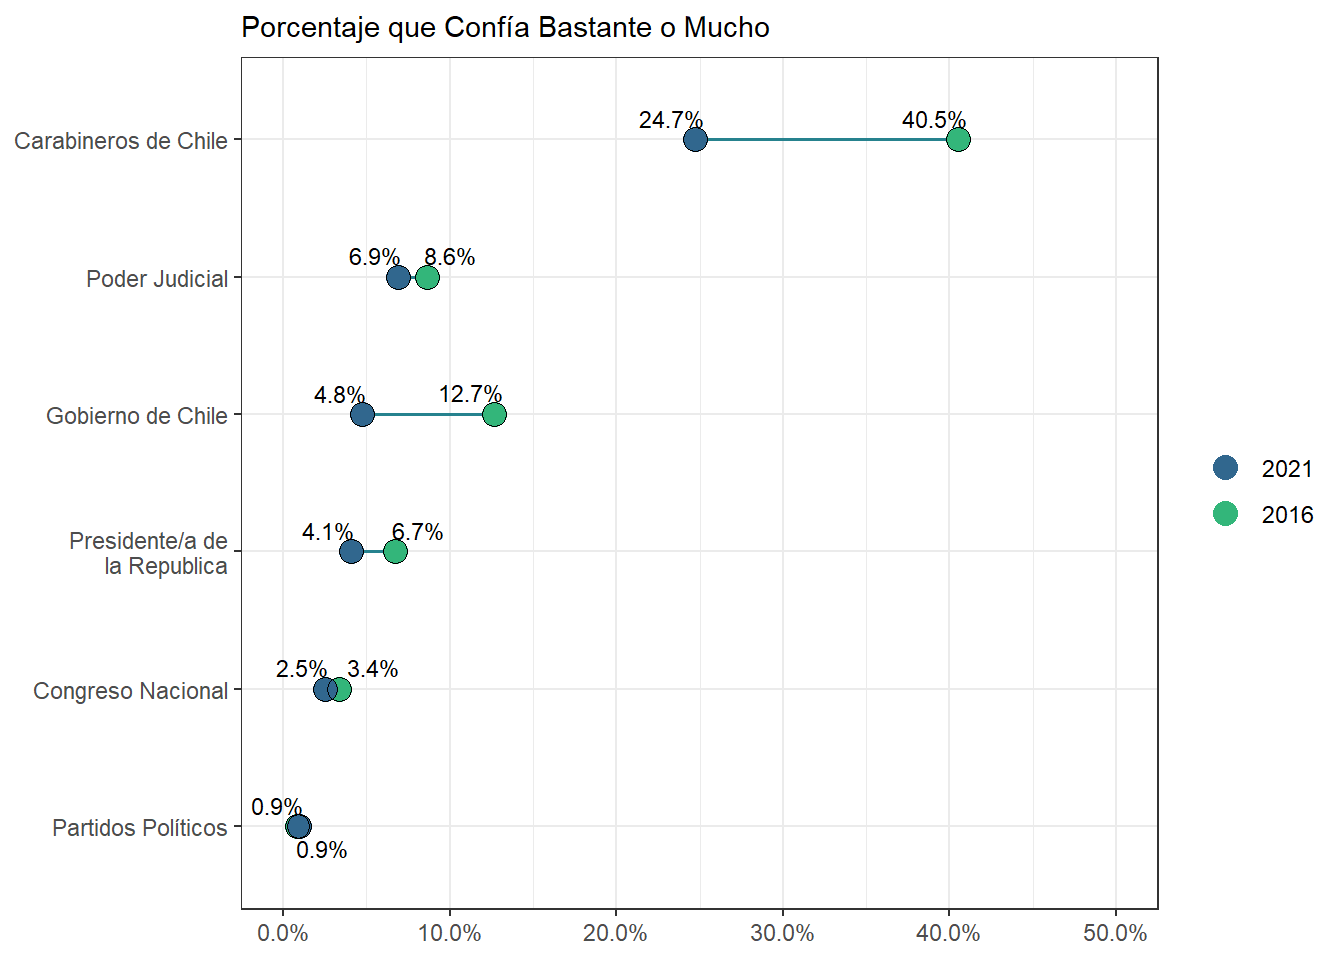
\includegraphics{reporte-elsoc_files/figure-latex/graf-cambio-confianza_instituciones-ola-1}

\}

\caption{Cambio en grado de confianza en instituciones (2016-2021)}

(\#fig:graf-cambio-confianza\_instituciones-ola)
\textbackslash end\{figure\}

\hypertarget{actitudes-hacia-la-democracia}{%
\section{Actitudes hacia la democracia}\label{actitudes-hacia-la-democracia}}

\textbackslash begin\{figure\}

\{\centering 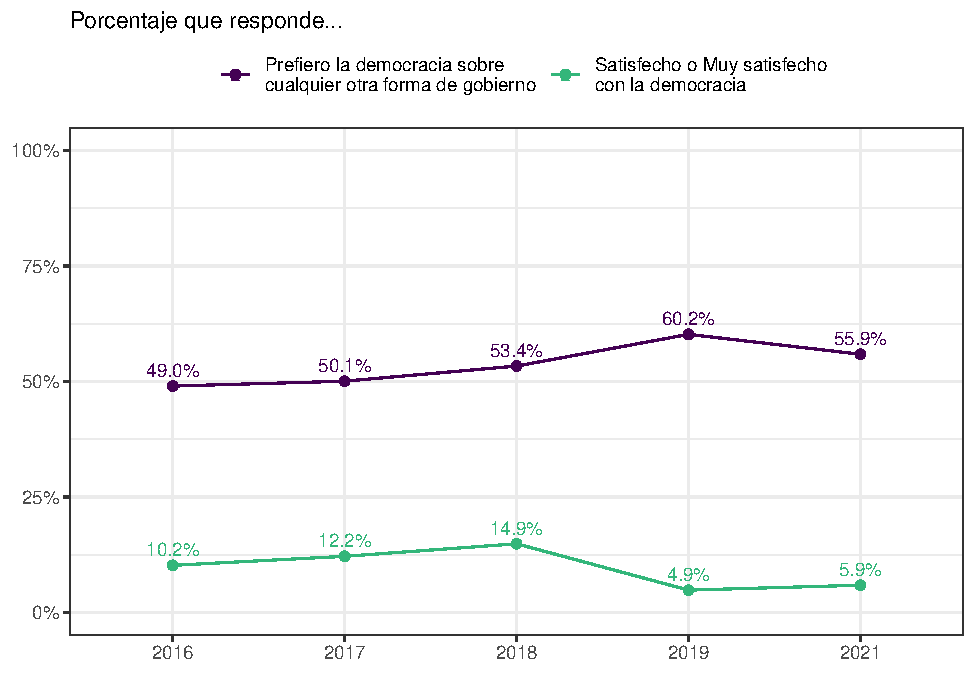
\includegraphics{reporte-elsoc_files/figure-latex/graf-preferencia_democracia-ola-1}

\}

\caption{Preferencia por y satisfacción con la democracia, según ola}

(\#fig:graf-preferencia\_democracia-ola)
\textbackslash end\{figure\}

\textbackslash begin\{figure\}

\{\centering 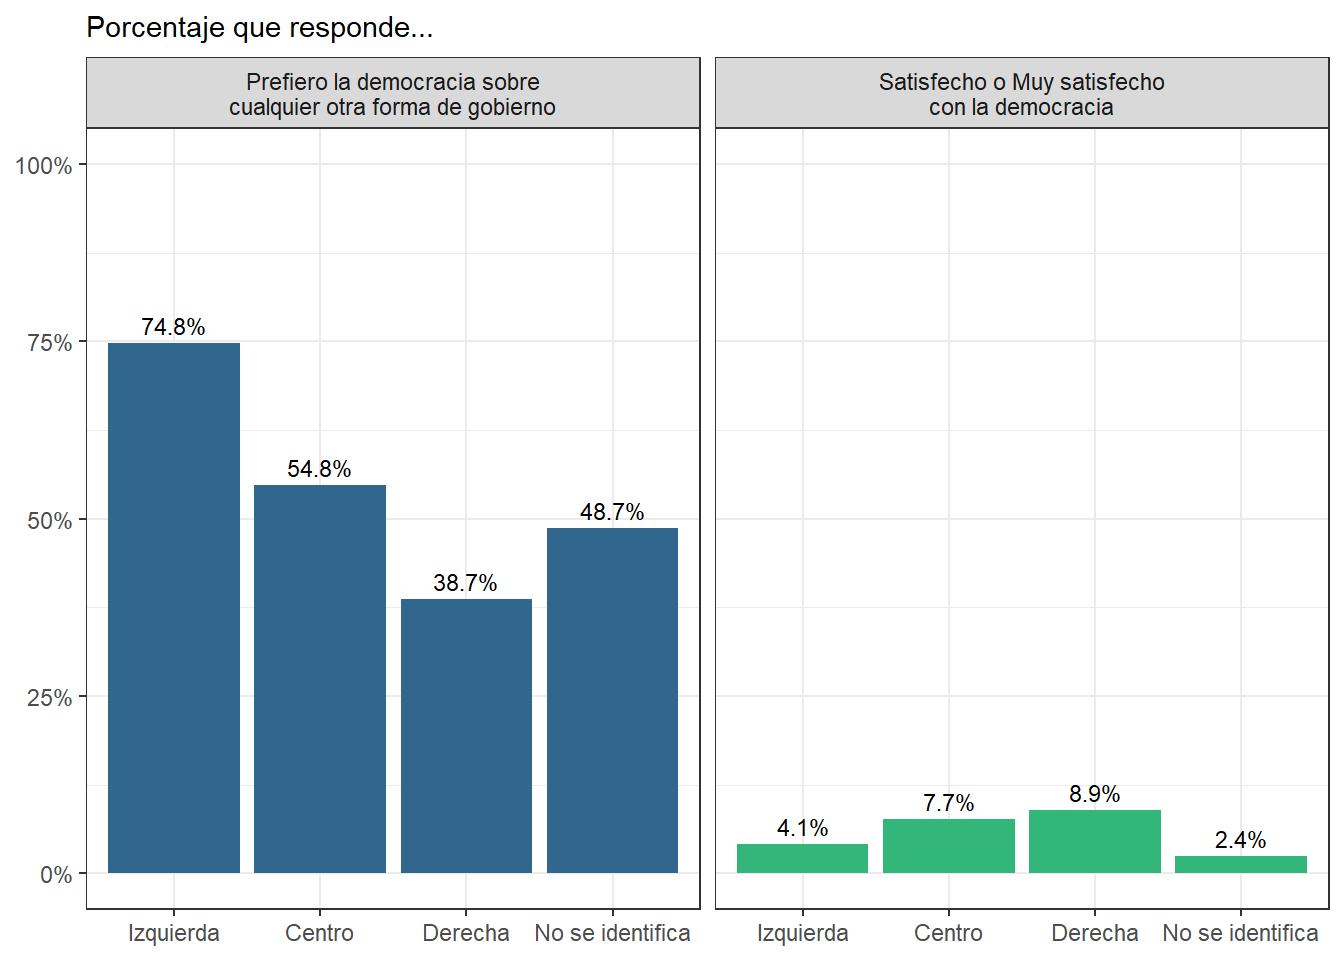
\includegraphics{reporte-elsoc_files/figure-latex/graf-preferencia_democracia-idpolitica-1}

\}

\caption{Preferencia por y satisfacción con la democracia (2021), según posición ideológica}

(\#fig:graf-preferencia\_democracia-idpolitica)
\textbackslash end\{figure\}

\textbackslash begin\{figure\}

\{\centering 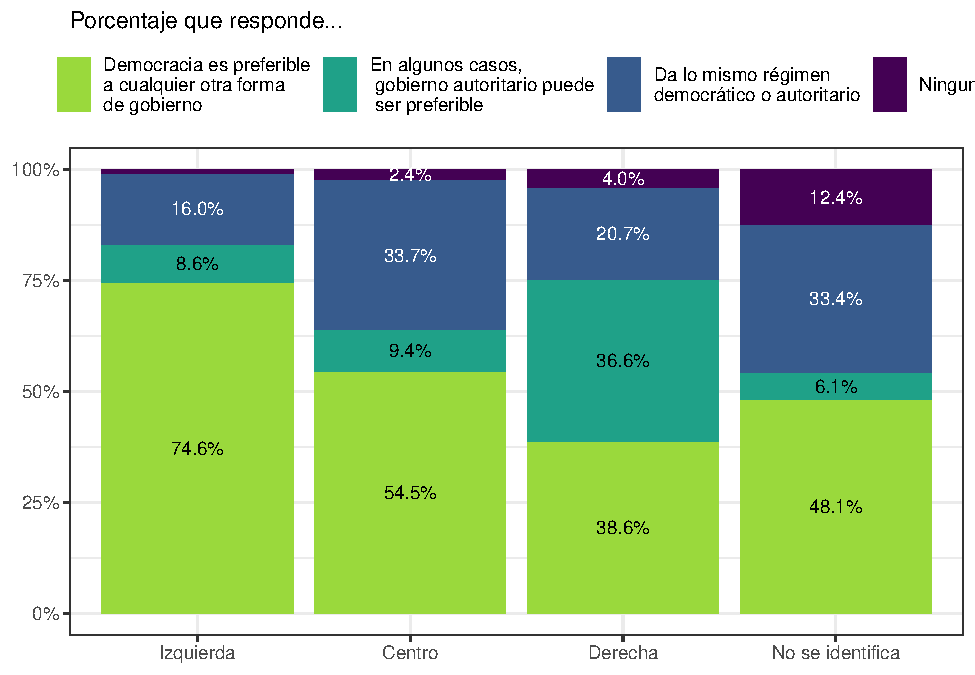
\includegraphics{reporte-elsoc_files/figure-latex/graf-preferencia_democracia2-idpolitica-1}

\}

\caption{Preferencia por la democracia (2021), según posición ideológica}

(\#fig:graf-preferencia\_democracia2-idpolitica)
\textbackslash end\{figure\}

\hypertarget{cambio-constitucional}{%
\section{Cambio constitucional}\label{cambio-constitucional}}

\textbackslash begin\{figure\}

\{\centering 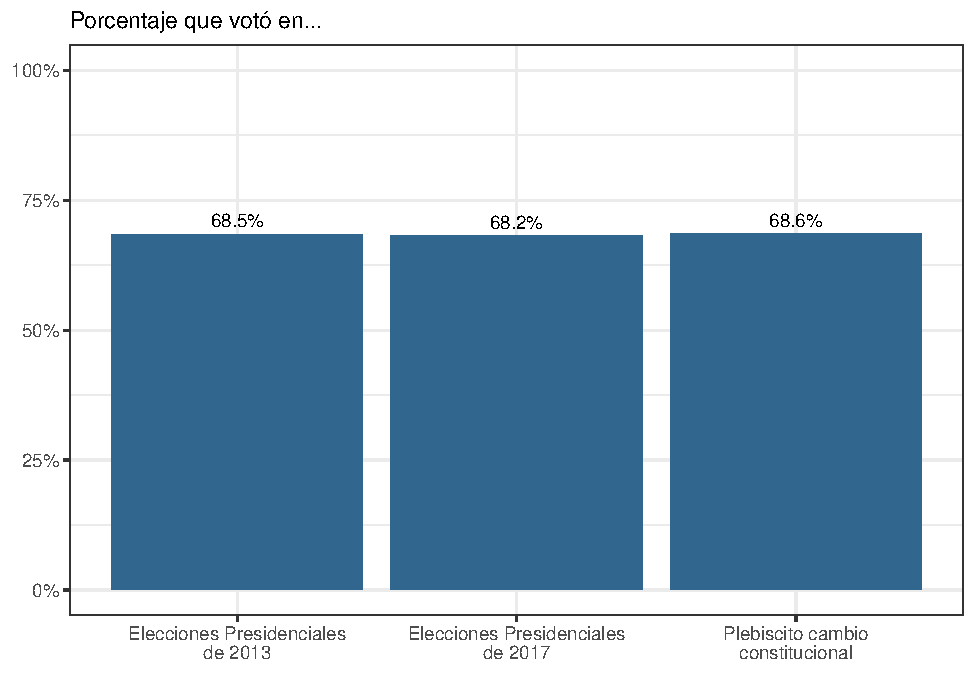
\includegraphics{reporte-elsoc_files/figure-latex/graf-particip_elect-ola-1}

\}

\caption{Participación electoral, según elección}

(\#fig:graf-particip\_elect-ola)
\textbackslash end\{figure\}

\begin{figure}

{\centering 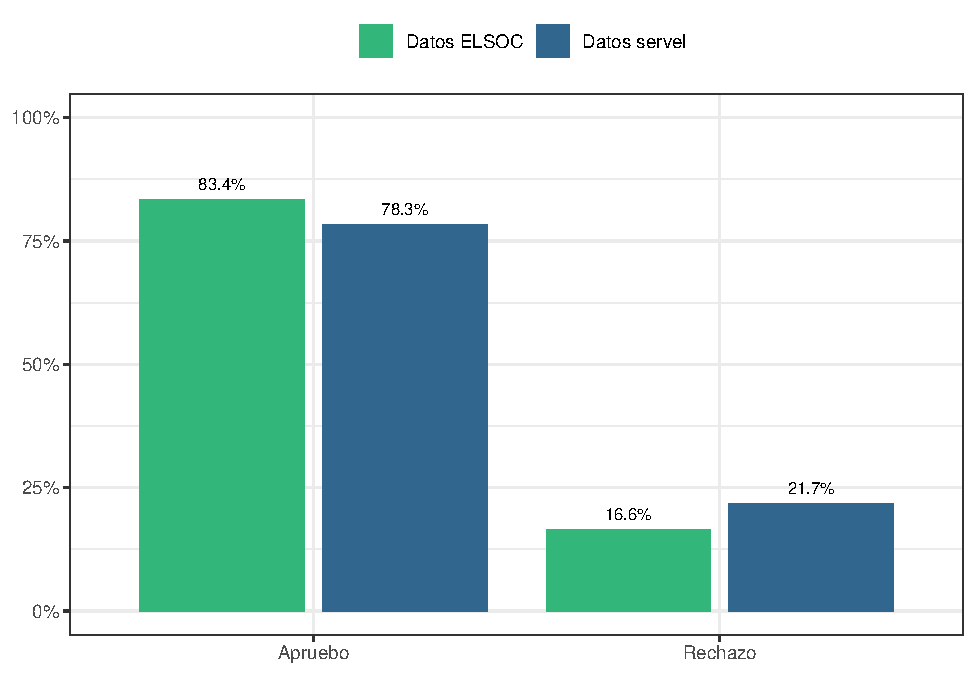
\includegraphics{reporte-elsoc_files/figure-latex/graf-servel-apruebo-1} 

}

\caption{Voto retrospectivo Plebiscito Nueva Constitucion}\label{fig:graf-servel-apruebo}
\end{figure}

\textbackslash begin\{figure\}

\{\centering 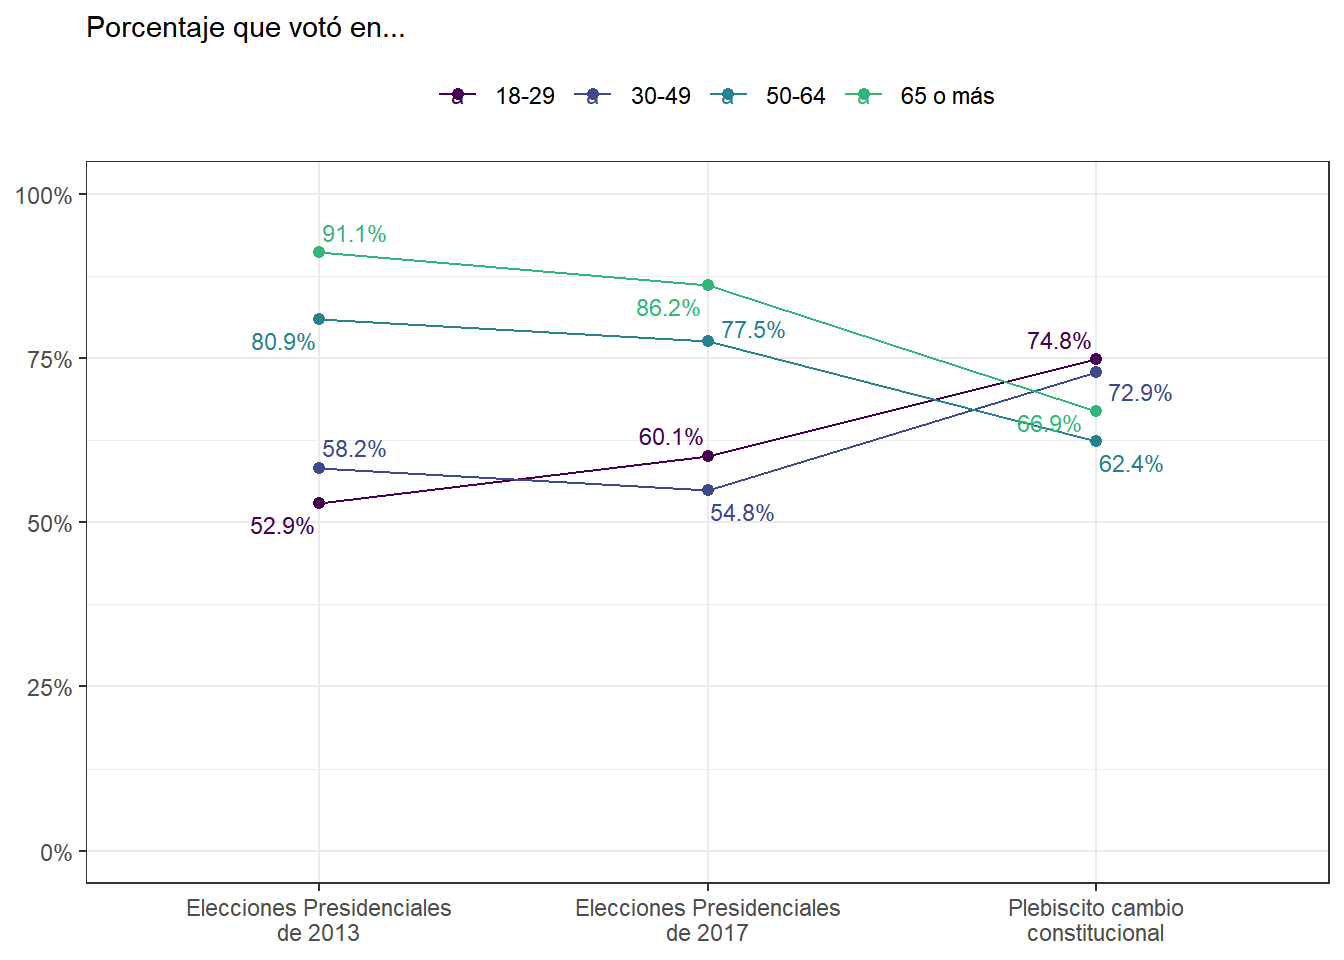
\includegraphics{reporte-elsoc_files/figure-latex/graf-particip_elect-olas-edad-1}

\}

\caption{Participación electoral, según tramo de edad}

(\#fig:graf-particip\_elect-olas-edad)
\textbackslash end\{figure\}

\textbackslash begin\{figure\}

\{\centering 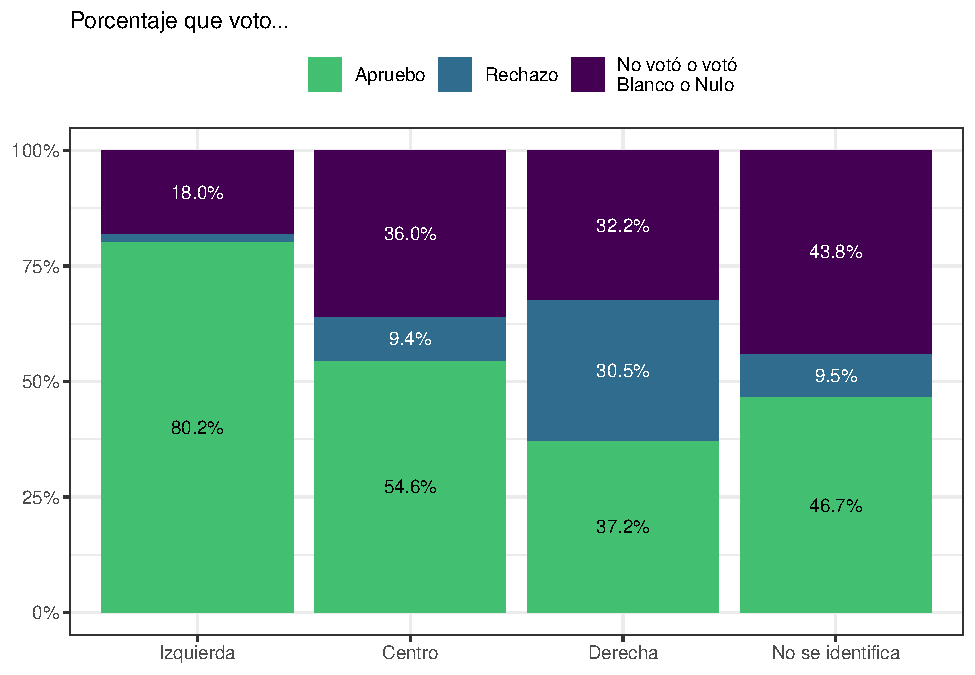
\includegraphics{reporte-elsoc_files/figure-latex/graf-voto_plebiscito-idpolitica-1}

\}

\caption{Voto en plebiscito de 2020, según identificación política}

(\#fig:graf-voto\_plebiscito-idpolitica)
\textbackslash end\{figure\}

\begin{figure}

{\centering 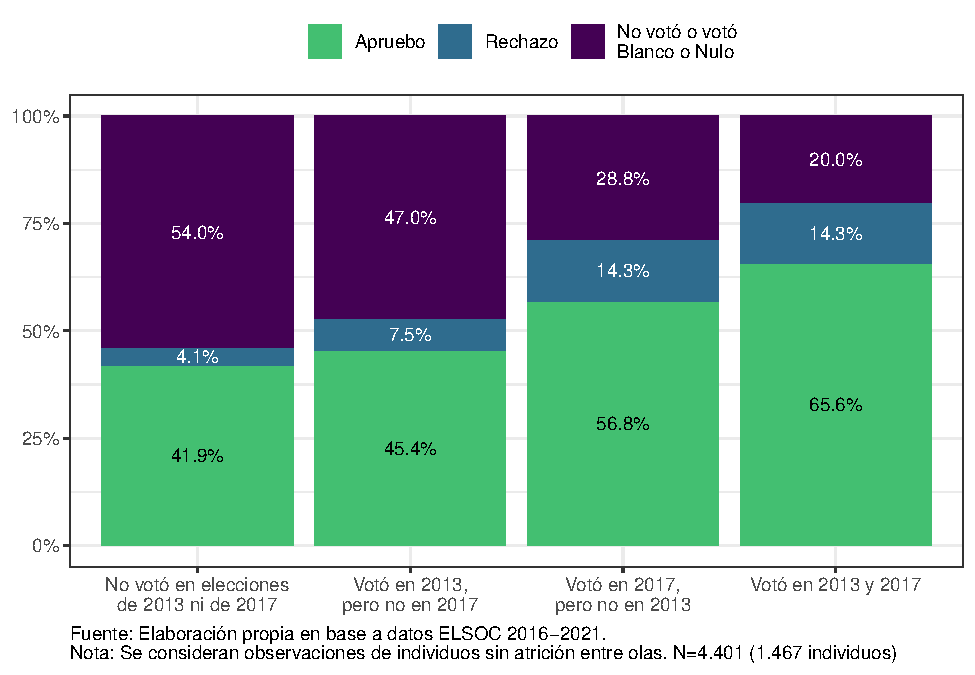
\includegraphics{reporte-elsoc_files/figure-latex/graf-voto-votoprevio-1} 

}

\caption{Voto en plebiscito de 2020, según voto en elecciones previas}\label{fig:graf-voto-votoprevio}
\end{figure}

\begin{figure}

{\centering 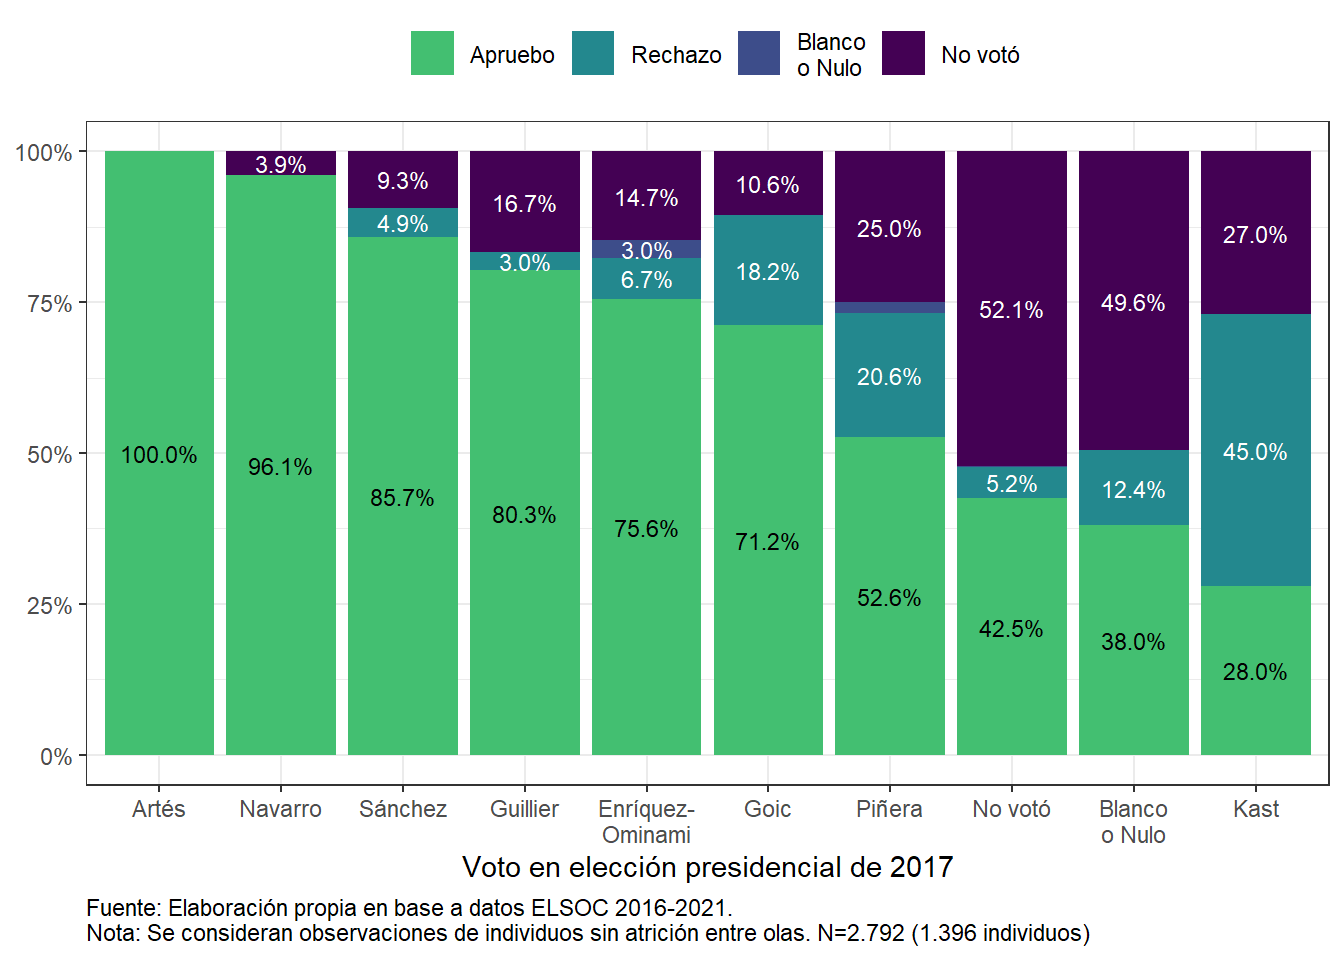
\includegraphics{reporte-elsoc_files/figure-latex/graf-voto-votopresi-1} 

}

\caption{Voto en plebiscito de 2020, según voto en elección presidencial de 2017}\label{fig:graf-voto-votopresi}
\end{figure}

\hypertarget{optimismo-constitucional}{%
\section{Optimismo constitucional}\label{optimismo-constitucional}}

\textbackslash begin\{figure\}

\{\centering 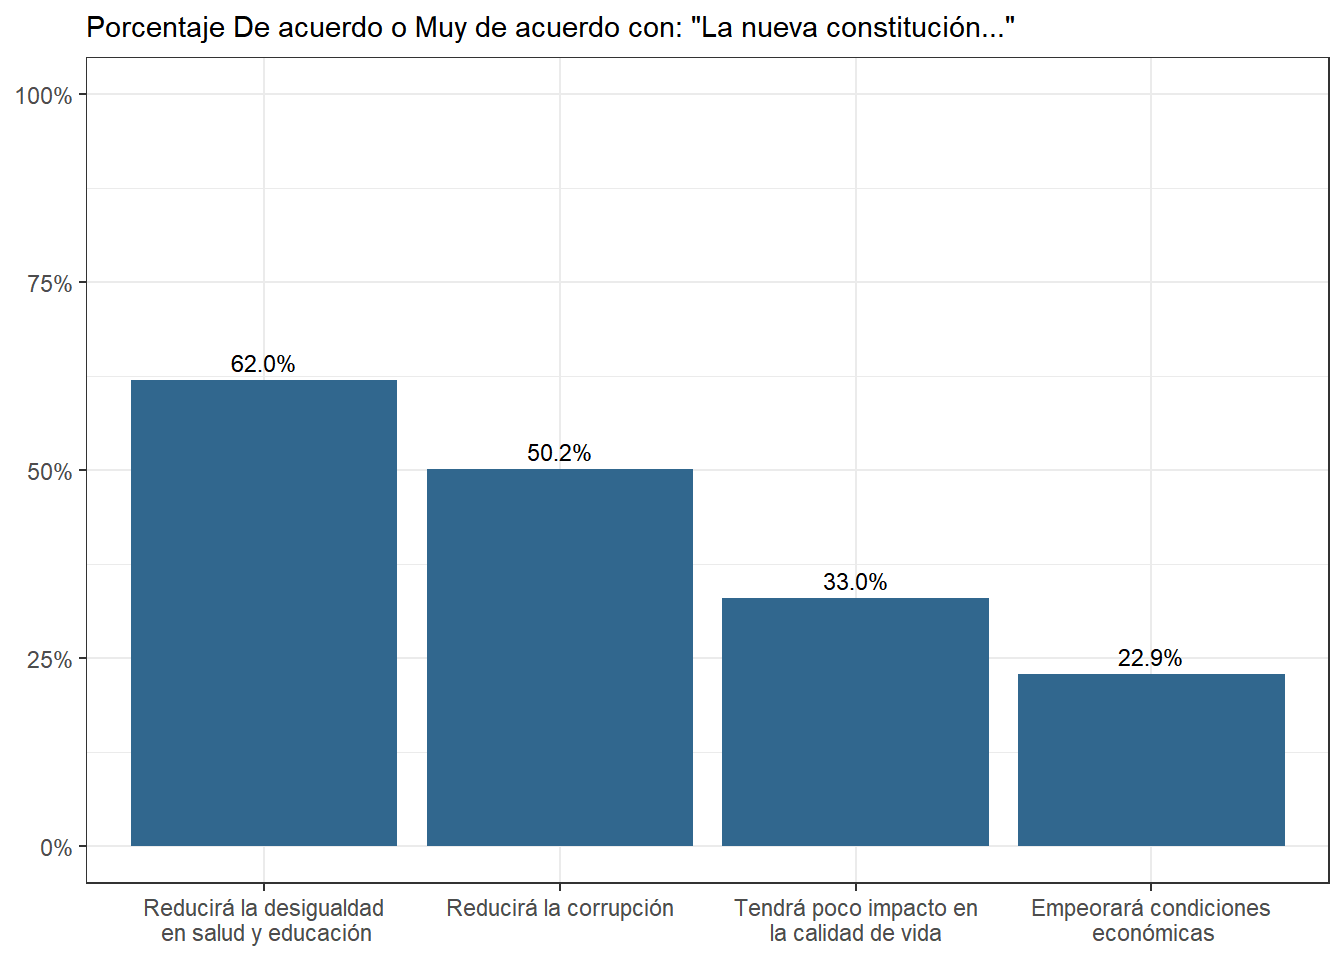
\includegraphics{reporte-elsoc_files/figure-latex/graf-optimismo_constitucional-1}

\}

\caption{Optimismo constitucional}

(\#fig:graf-optimismo\_constitucional)
\textbackslash end\{figure\}

\textbackslash begin\{figure\}

\{\centering 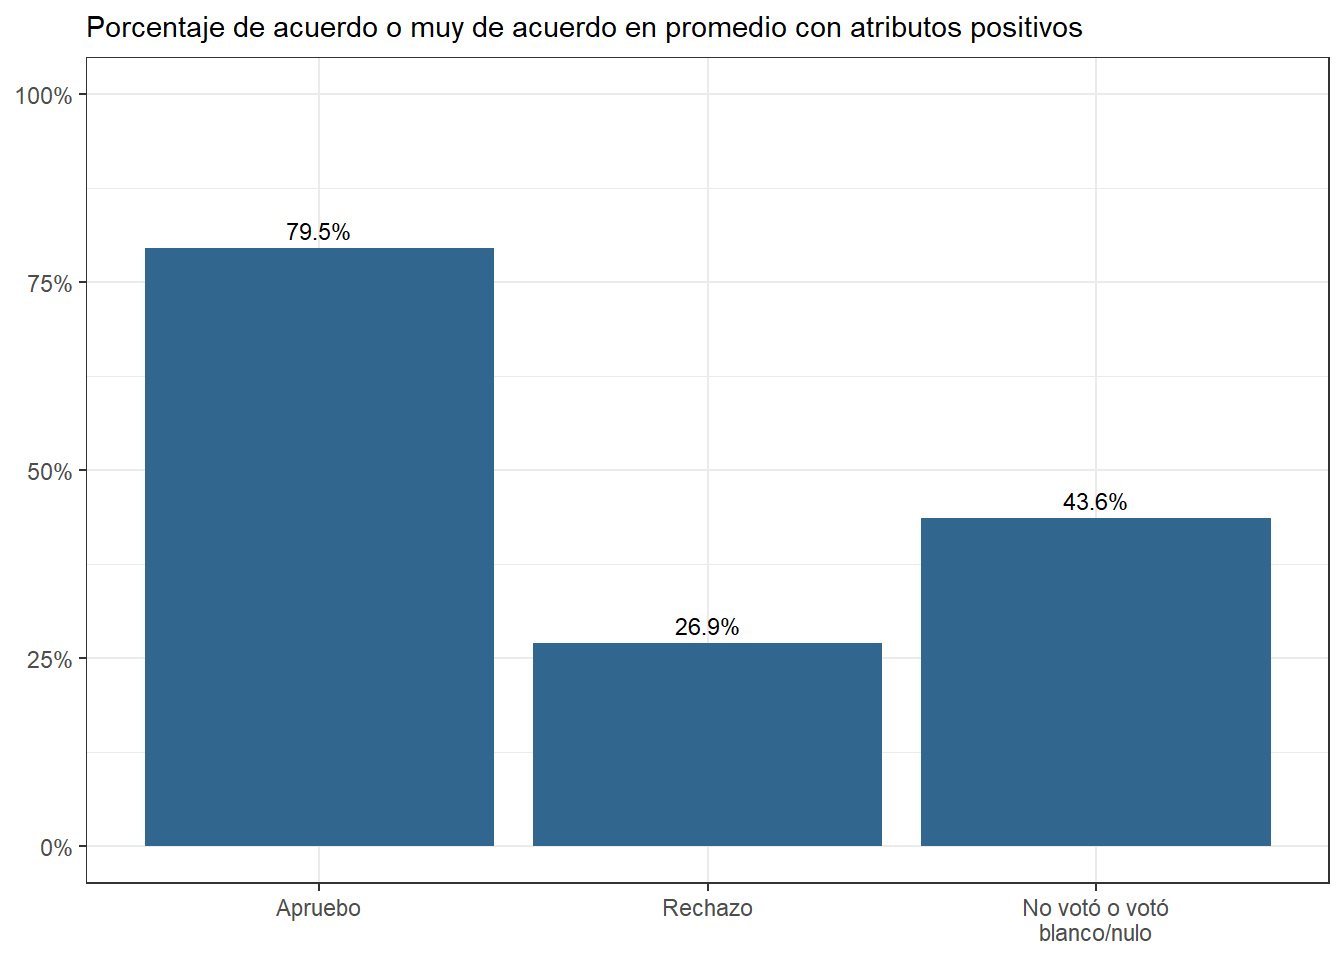
\includegraphics{reporte-elsoc_files/figure-latex/graf-optimismo_constitucional-voto_plebiscito-1}

\}

\caption{Optimismo constitucional, según voto en plebiscito de 2020}

(\#fig:graf-optimismo\_constitucional-voto\_plebiscito)
\textbackslash end\{figure\}

\textbackslash begin\{figure\}

\{\centering 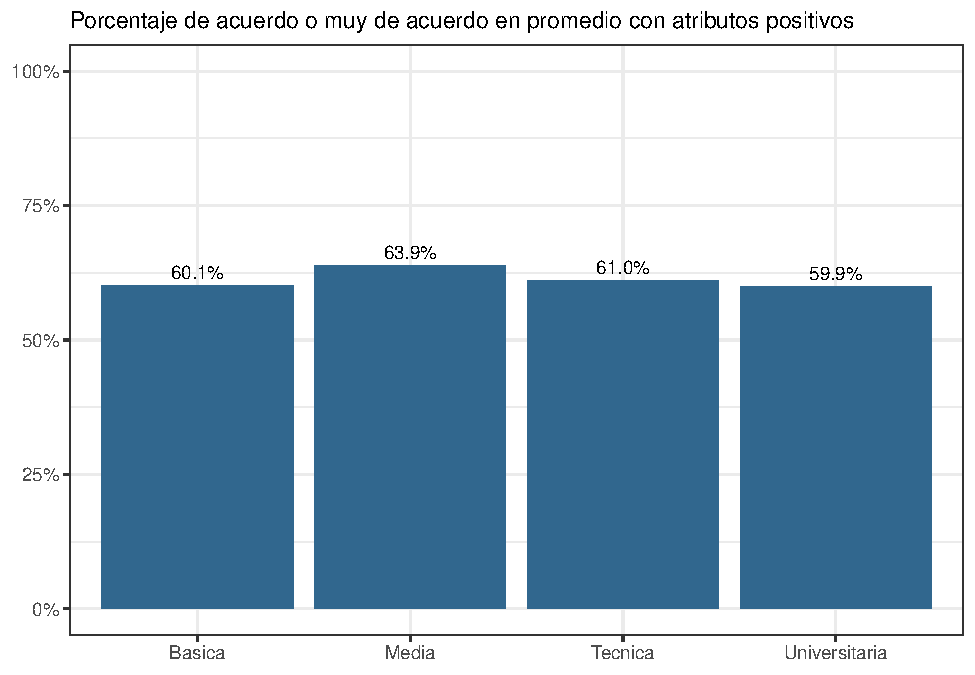
\includegraphics{reporte-elsoc_files/figure-latex/graf-optimismo_constitucional-educ-1}

\}

\caption{Optimismo constitucional, según nivel educacional}

(\#fig:graf-optimismo\_constitucional-educ)
\textbackslash end\{figure\}

\textbackslash begin\{figure\}

\{\centering 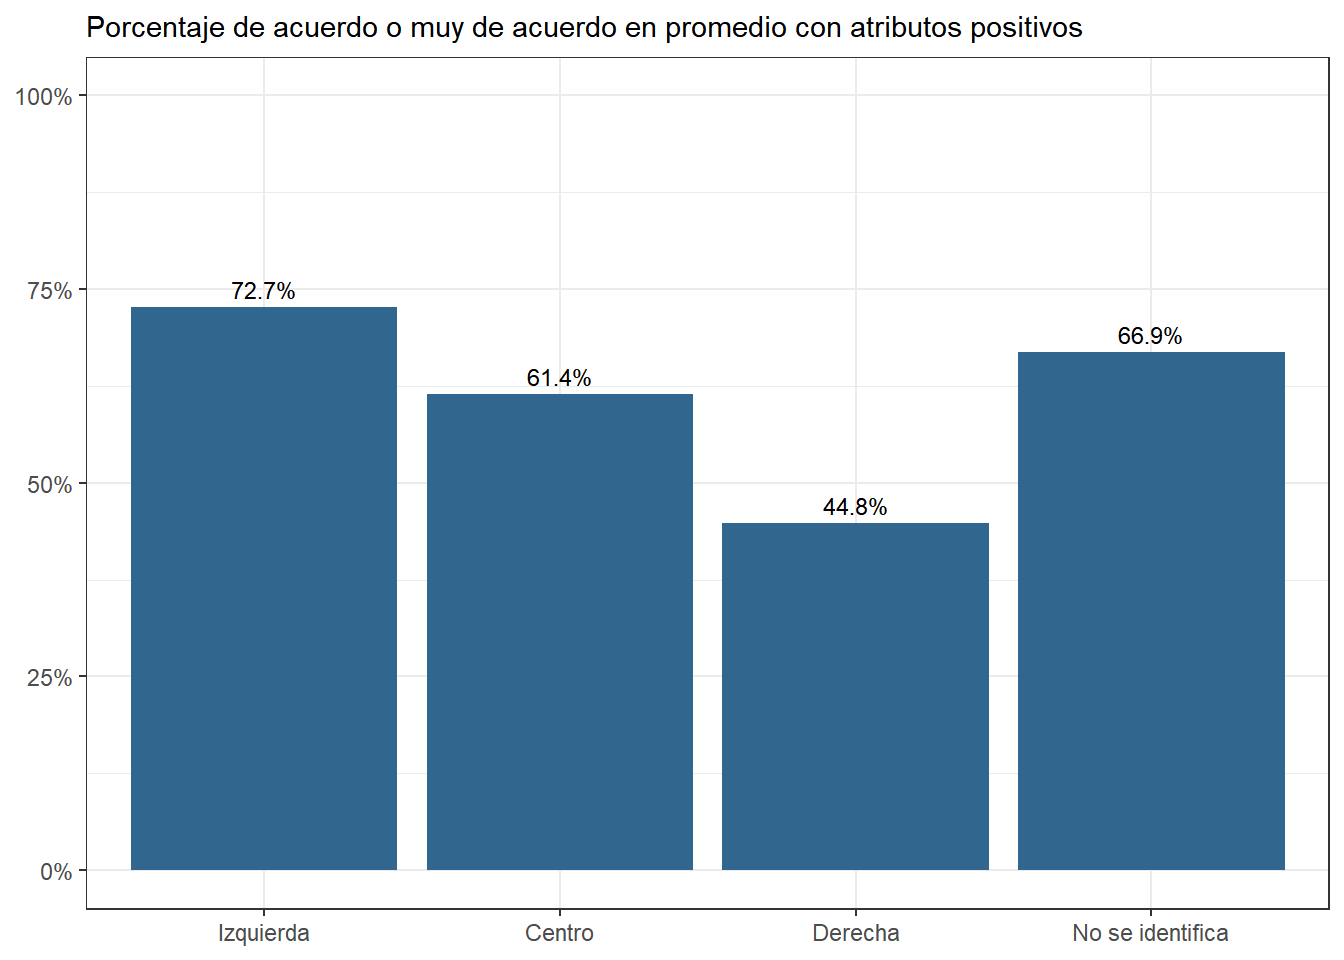
\includegraphics{reporte-elsoc_files/figure-latex/graf-optimismo_constitucional-idpolitica-1}

\}

\caption{Optimismo constitucional, según identificación política}

(\#fig:graf-optimismo\_constitucional-idpolitica)
\textbackslash end\{figure\}

\hypertarget{temas-de-salud-mental-y-bienestar}{%
\chapter{Temas de salud mental y bienestar}\label{temas-de-salud-mental-y-bienestar}}

\hypertarget{salud-mental-y-bienestar-de-la-poblaciuxf3n}{%
\section{Salud mental y bienestar de la población}\label{salud-mental-y-bienestar-de-la-poblaciuxf3n}}

\hypertarget{cuxf3mo-ha-cambiado-la-salud-mental-y-nivel-de-bienestar-de-la-poblaciuxf3n}{%
\subsection{¿Cómo ha cambiado la salud mental y nivel de bienestar de la población?}\label{cuxf3mo-ha-cambiado-la-salud-mental-y-nivel-de-bienestar-de-la-poblaciuxf3n}}

\begin{center}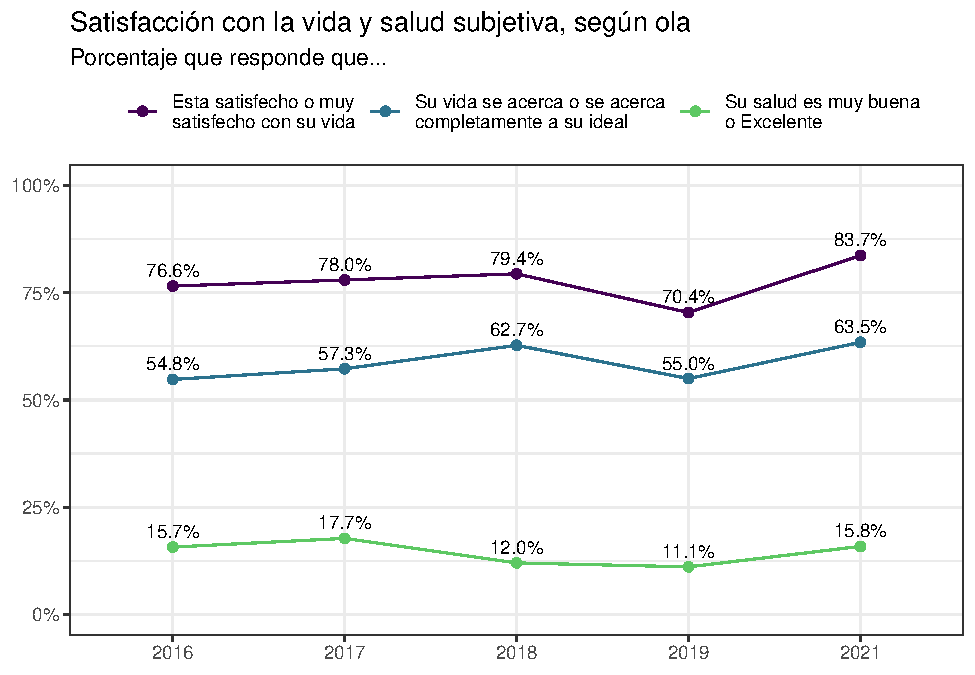
\includegraphics{reporte-elsoc_files/figure-latex/unnamed-chunk-1-1} \end{center}

\begin{center}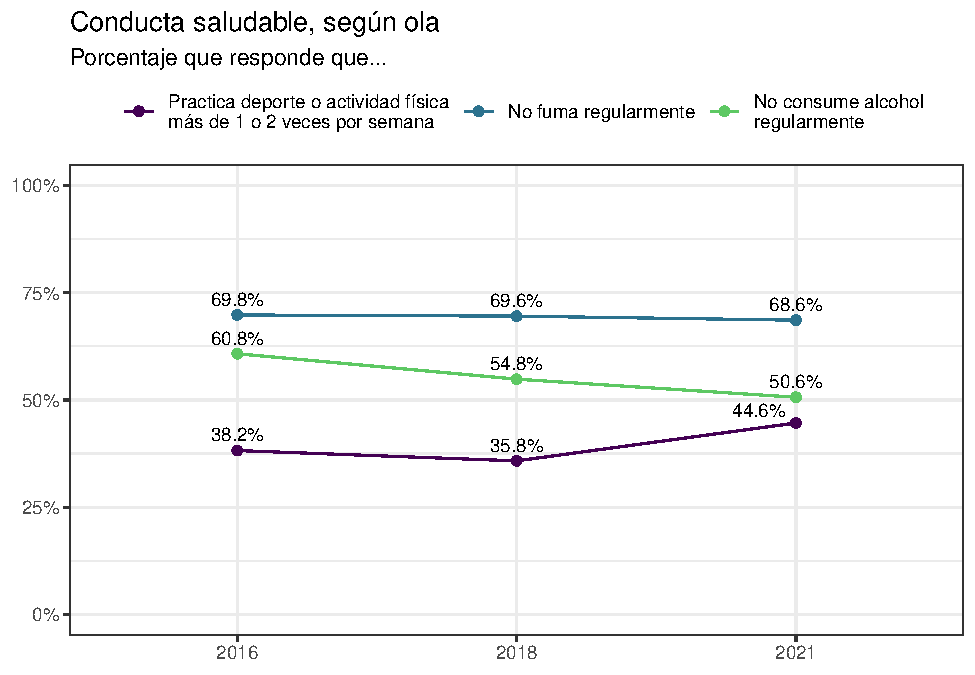
\includegraphics{reporte-elsoc_files/figure-latex/unnamed-chunk-2-1} \end{center}

\begin{center}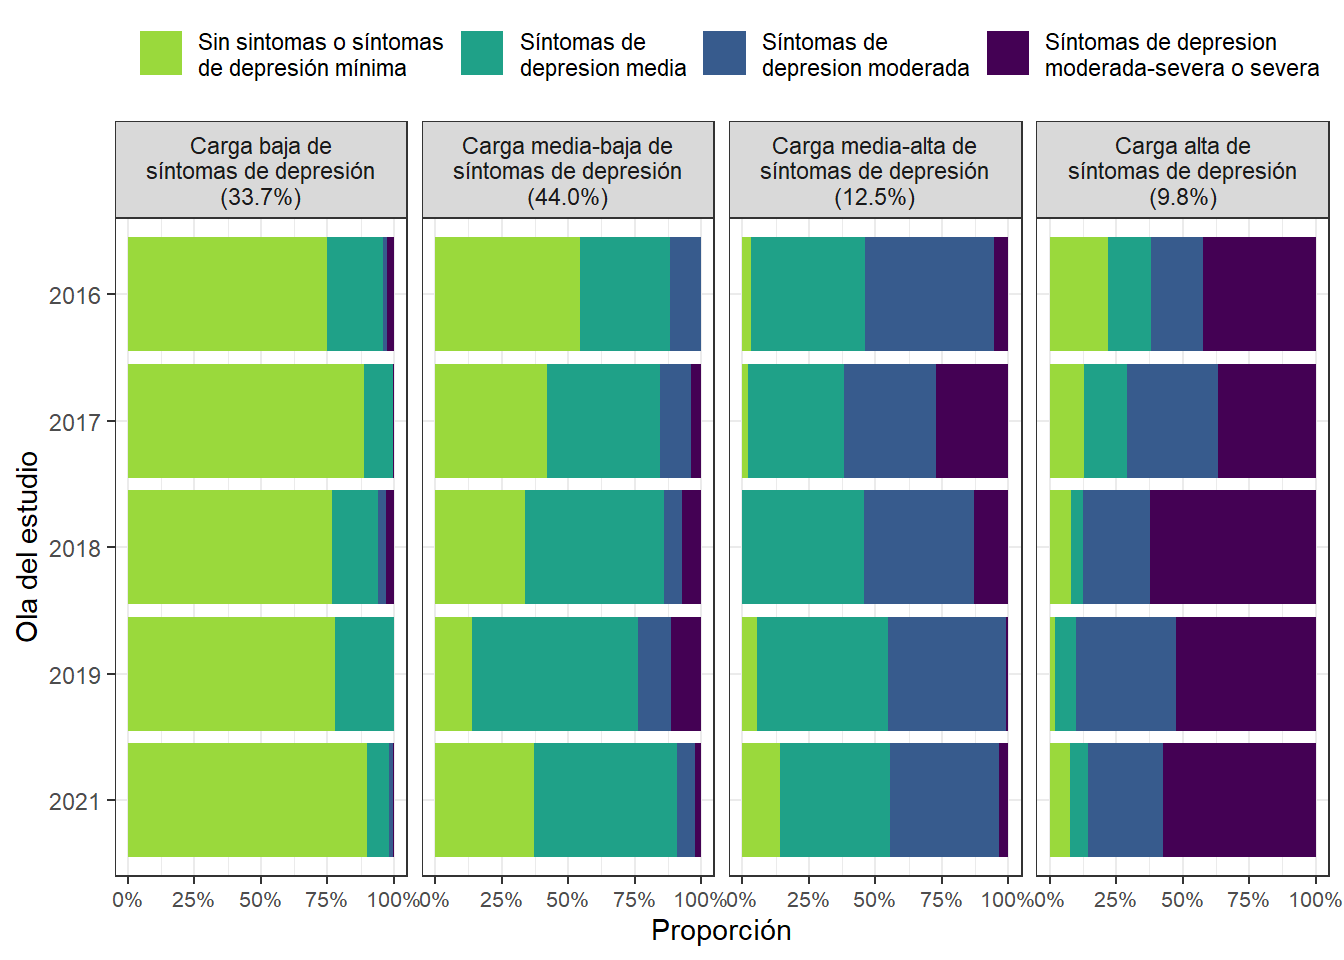
\includegraphics{reporte-elsoc_files/figure-latex/unnamed-chunk-3-1} \end{center}

\begin{center}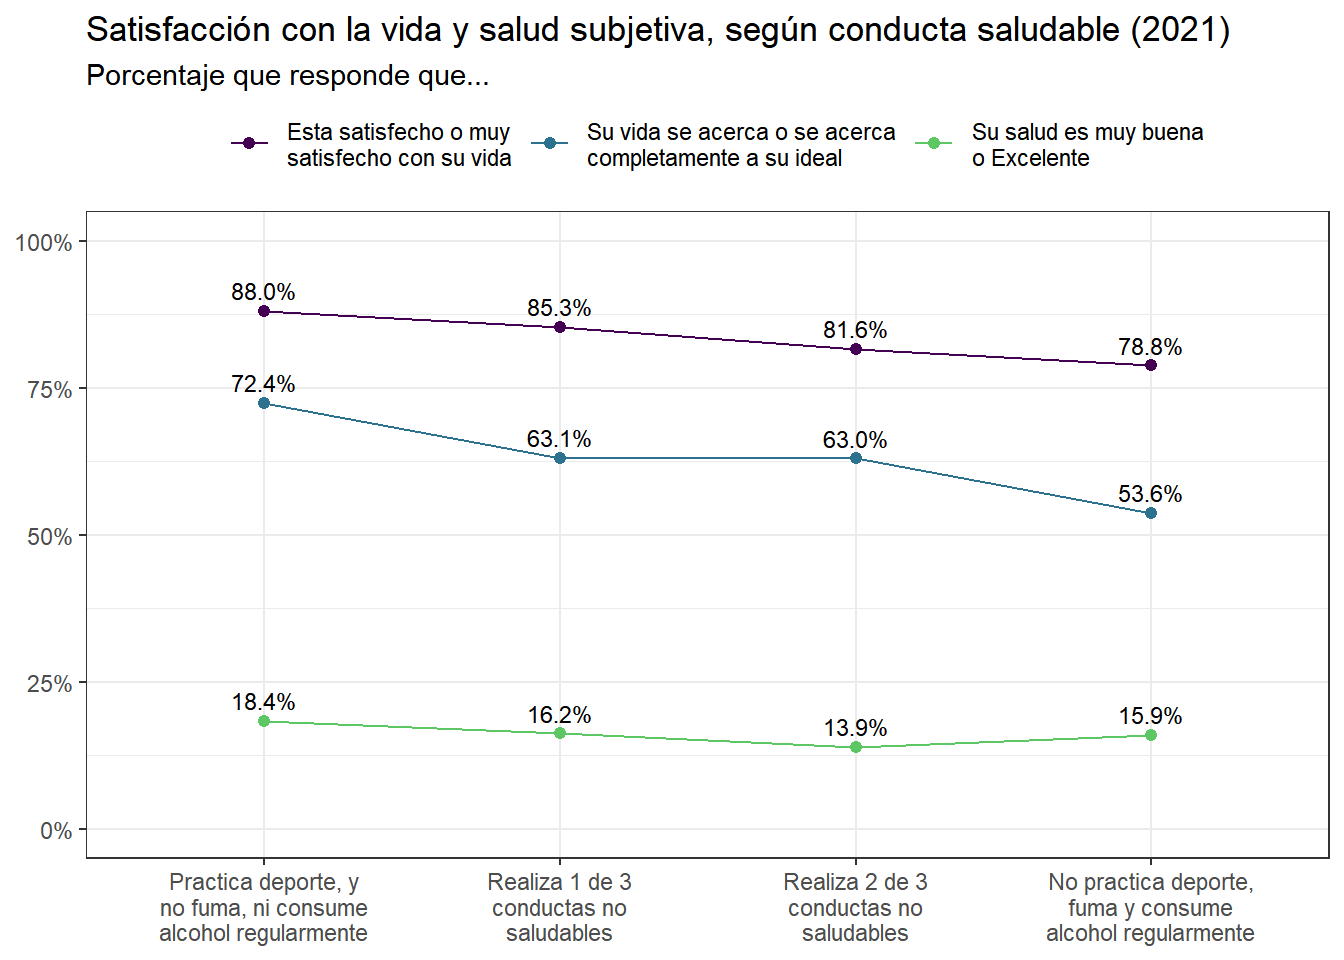
\includegraphics{reporte-elsoc_files/figure-latex/unnamed-chunk-4-1} \end{center}

\hypertarget{sintomatologuxeda-depresiva}{%
\subsection{Sintomatología depresiva}\label{sintomatologuxeda-depresiva}}

\begin{center}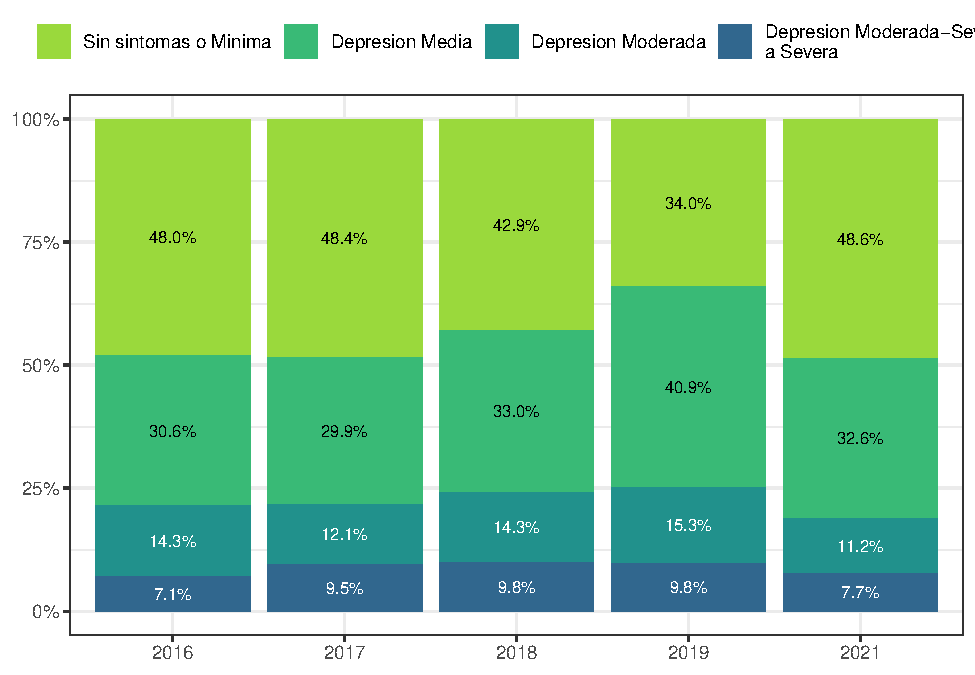
\includegraphics{reporte-elsoc_files/figure-latex/depre-wave-1} \end{center}

\begin{center}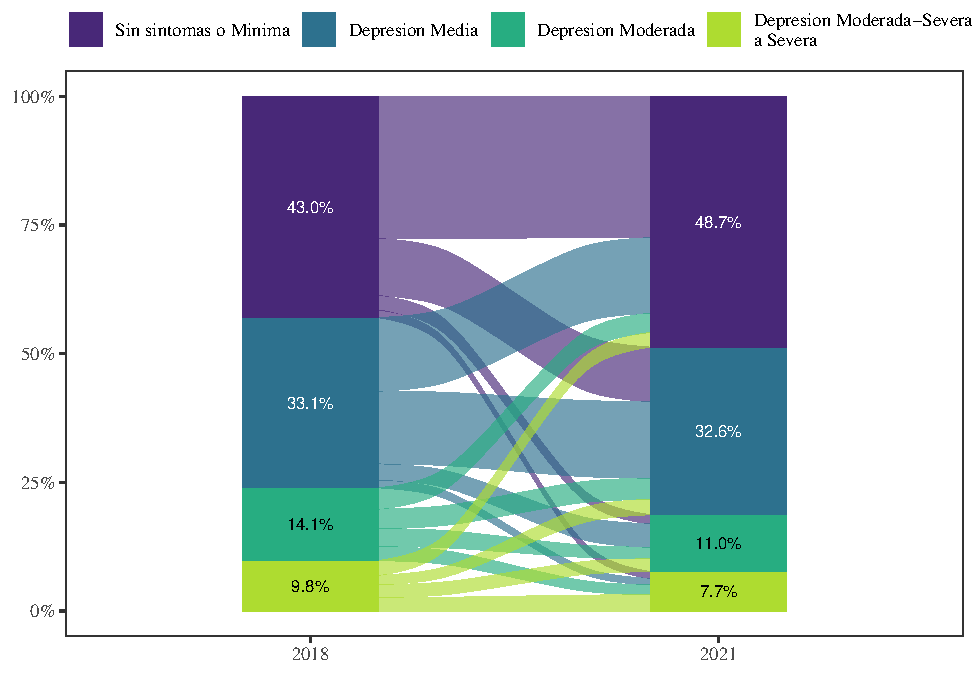
\includegraphics{reporte-elsoc_files/figure-latex/depre-sexo-1} \end{center}

\begin{center}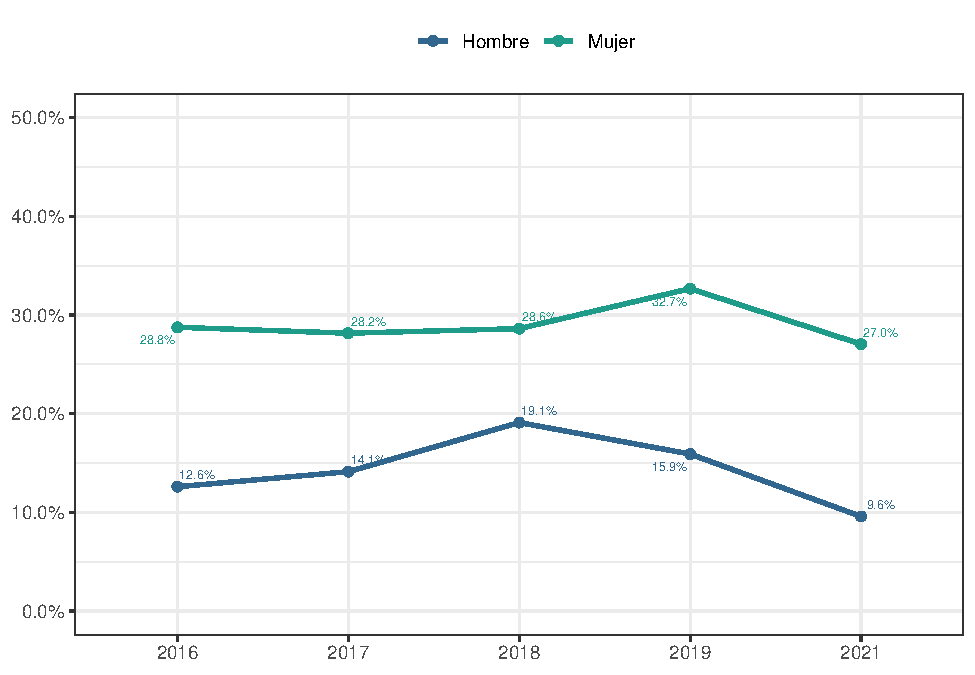
\includegraphics{reporte-elsoc_files/figure-latex/depre-year-sexo-1} \end{center}

\begin{center}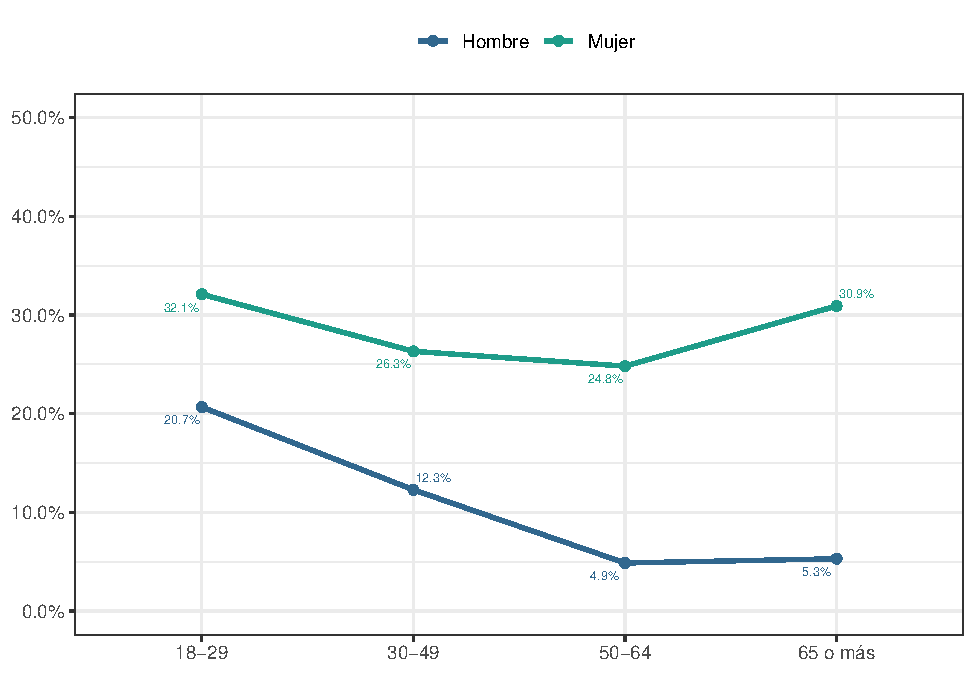
\includegraphics{reporte-elsoc_files/figure-latex/depre-edad-sexo-1} \end{center}

\begin{center}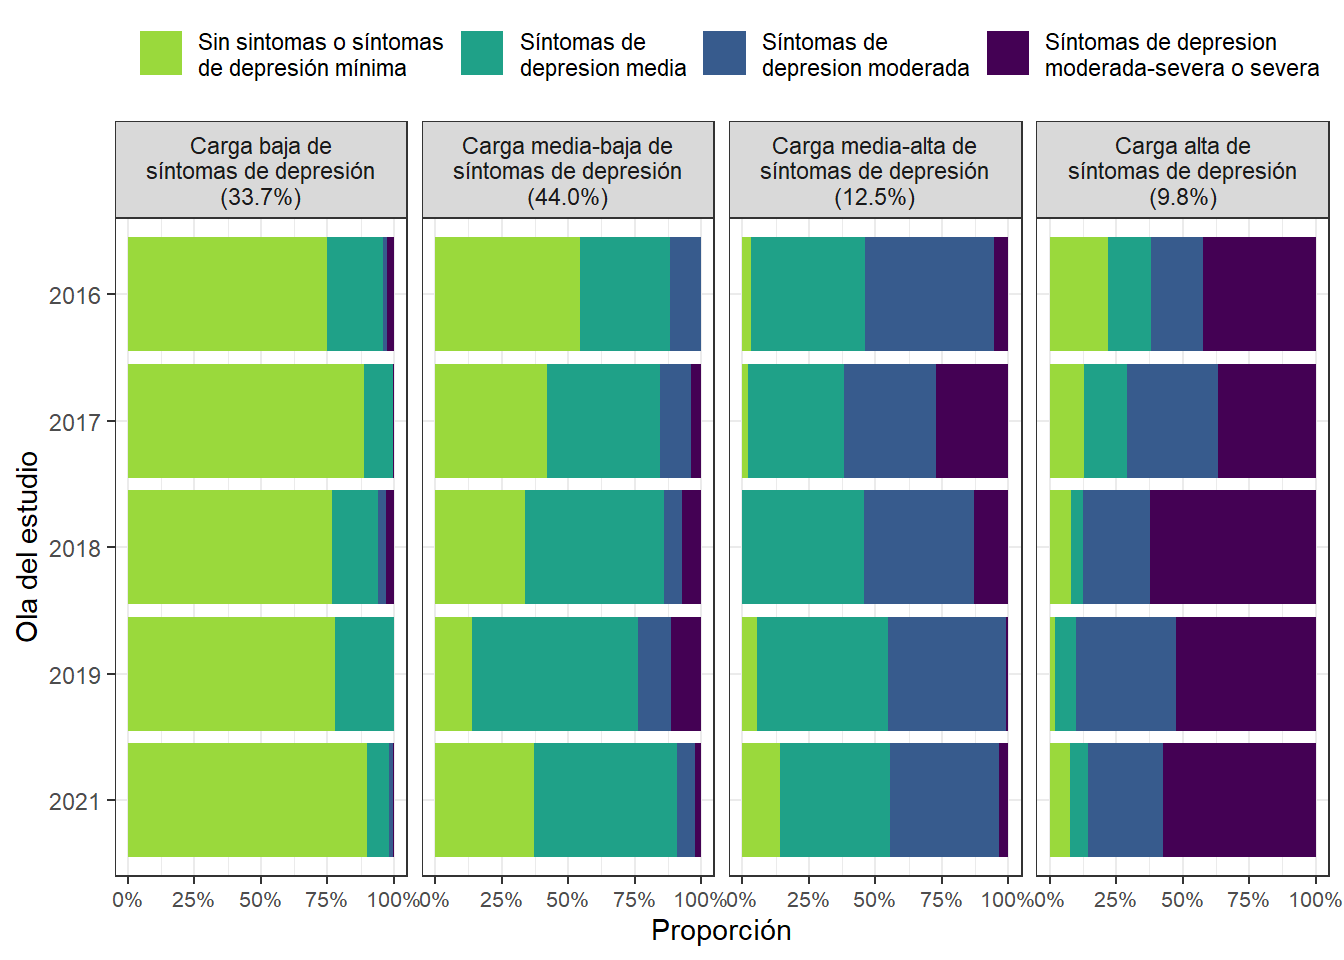
\includegraphics{reporte-elsoc_files/figure-latex/unnamed-chunk-5-1} \end{center}

\begin{center}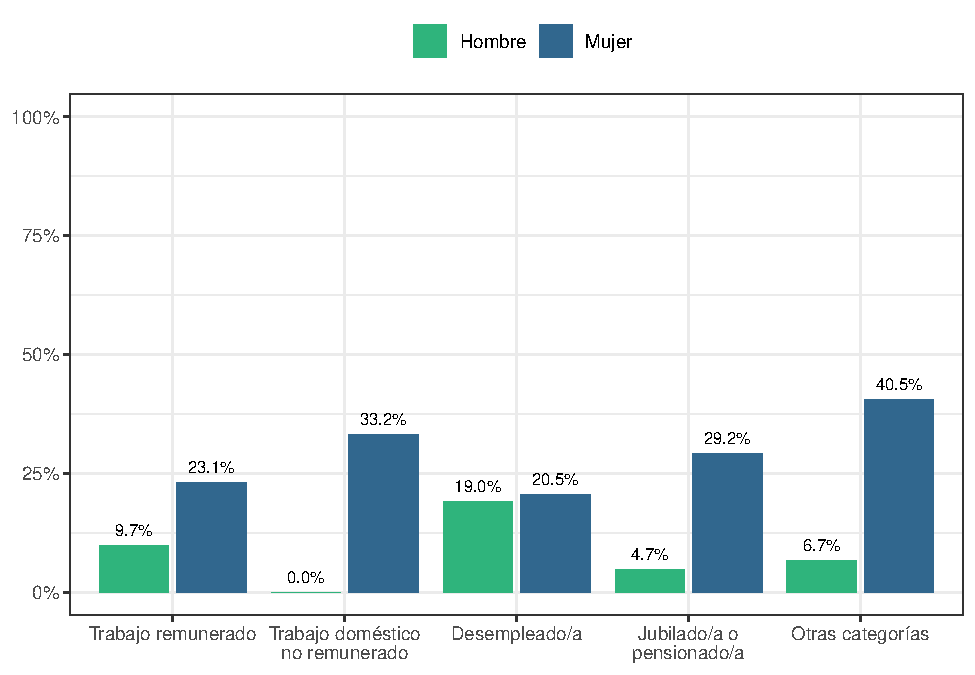
\includegraphics{reporte-elsoc_files/figure-latex/depre-labstat-1} \end{center}

En 2021 no hay hombres en la categoría Trabajo doméstico no remunerado \(^{*}\)

\hypertarget{covid---19}{%
\section{COVID - 19}\label{covid---19}}

\begin{center}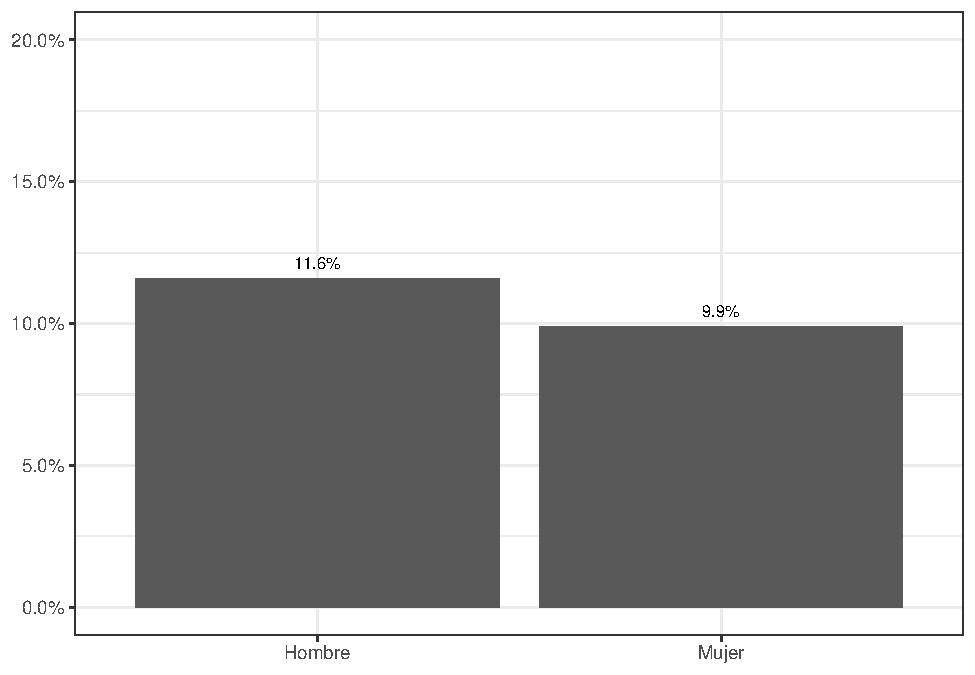
\includegraphics{reporte-elsoc_files/figure-latex/covid-sexo-1} \end{center}

\begin{center}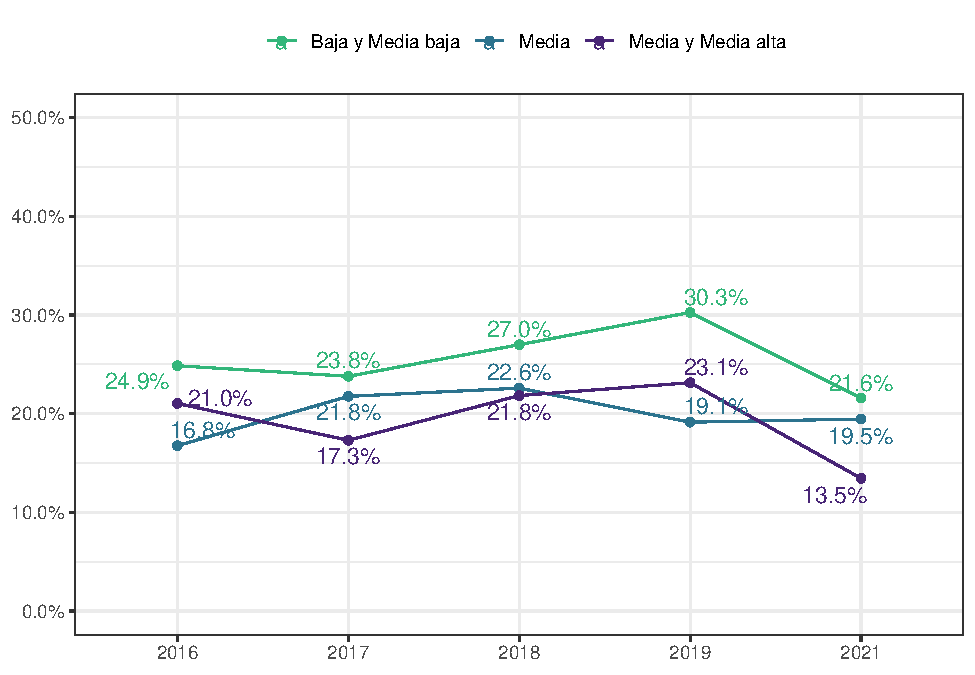
\includegraphics{reporte-elsoc_files/figure-latex/depre clase.sub-1} \end{center}

\begin{center}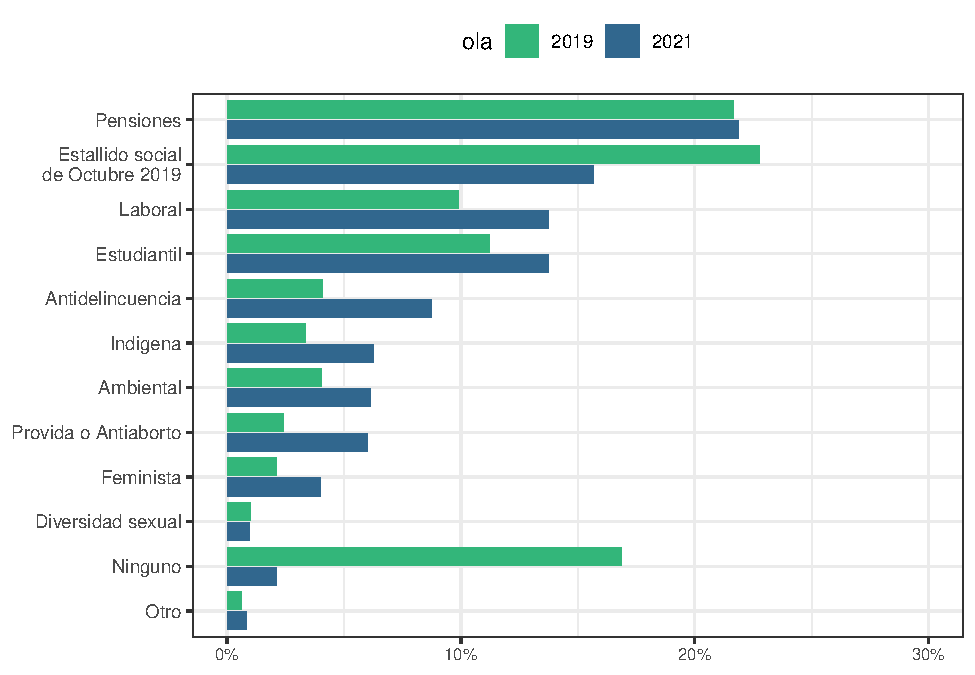
\includegraphics{reporte-elsoc_files/figure-latex/unnamed-chunk-6-1} \end{center}

\hypertarget{cuarentenas}{%
\subsection{Cuarentenas}\label{cuarentenas}}

\begin{center}\includegraphics{reporte-elsoc_files/figure-latex/hist-fecha-2021-1} \end{center}

\begin{center}\includegraphics{reporte-elsoc_files/figure-latex/unnamed-chunk-7-1} \end{center}

\begin{center}\includegraphics{reporte-elsoc_files/figure-latex/unnamed-chunk-8-1} \end{center}

\begin{verbatim}
## 1 variables were not found in the dataset: ola
\end{verbatim}

\begin{center}\includegraphics{reporte-elsoc_files/figure-latex/unnamed-chunk-9-1} \end{center}

\begin{verbatim}
## 1 variables were not found in the dataset: ola
\end{verbatim}

\begin{center}\includegraphics{reporte-elsoc_files/figure-latex/unnamed-chunk-10-1} \end{center}

\hypertarget{grado-de-acuerdo-con-actividad-econuxf3mica-versus-salud-puxfablica-seguxfan-identificaciuxf3n-poluxedtica-el-auxf1o-2021}{%
\subsection{Grado de acuerdo con actividad económica versus salud pública según identificación política el año 2021}\label{grado-de-acuerdo-con-actividad-econuxf3mica-versus-salud-puxfablica-seguxfan-identificaciuxf3n-poluxedtica-el-auxf1o-2021}}

\begin{verbatim}
## 1 variables were not found in the dataset: c37_09
\end{verbatim}

\begin{center}\includegraphics{reporte-elsoc_files/figure-latex/unnamed-chunk-11-1} \end{center}

\begin{center}\includegraphics{reporte-elsoc_files/figure-latex/unnamed-chunk-12-1} \end{center}

\hypertarget{estruxe9s-financiero}{%
\section{Estrés Financiero}\label{estruxe9s-financiero}}

\begin{center}\includegraphics{reporte-elsoc_files/figure-latex/satisfaccion-wave-1} \end{center}

\begin{center}\includegraphics{reporte-elsoc_files/figure-latex/satisfaccion-retiro-1} \end{center}

\begin{center}\includegraphics{reporte-elsoc_files/figure-latex/clase.sub-benef.estatal-1} \end{center}

\begin{center}\includegraphics{reporte-elsoc_files/figure-latex/clase.sub.hij-1erretiro-1} \end{center}

\begin{center}\includegraphics{reporte-elsoc_files/figure-latex/endeud-1retiro-1} \end{center}

\begin{center}\includegraphics{reporte-elsoc_files/figure-latex/endeud-2retiro-1} \end{center}

\begin{center}\includegraphics{reporte-elsoc_files/figure-latex/deuda-retiro1-1} \end{center}

\hypertarget{distanciamiento-y-comportamiento-prosocial-en-pandemia}{%
\section{Distanciamiento y comportamiento prosocial en pandemia}\label{distanciamiento-y-comportamiento-prosocial-en-pandemia}}

\begin{figure}

{\centering \includegraphics{reporte-elsoc_files/figure-latex/dist-total-1} 

}

\caption{¿En qué medida usted ha seguido la recomendación de quedarse en su hogar, manteniendo el aislamiento social? (2021).}\label{fig:dist-total}
\end{figure}

\begin{figure}

{\centering \includegraphics{reporte-elsoc_files/figure-latex/dist-quintil-1} 

}

\caption{¿En qué medida usted ha seguido la recomendación de quedarse en su hogar, manteniendo el aislamiento social? según quintil de ingreso. Suma de respuestas "Frecuente o "Muy frecuentemente" (2021).}\label{fig:dist-quintil}
\end{figure}

\begin{figure}

{\centering \includegraphics{reporte-elsoc_files/figure-latex/dist-edad-1} 

}

\caption{¿En qué medida usted ha seguido la recomendación de quedarse en su hogar, manteniendo el aislamiento social? según edad. Suma de respuestas "Frecuente o "Muy frecuentemente" (2021).}\label{fig:dist-edad}
\end{figure}

\begin{figure}

{\centering \includegraphics{reporte-elsoc_files/figure-latex/dist-estrato-1} 

}

\caption{¿En qué medida usted ha seguido la recomendación de quedarse en su hogar, manteniendo el aislamiento social? según estrato muestral (2021).}\label{fig:dist-estrato}
\end{figure}

\begin{figure}

{\centering \includegraphics{reporte-elsoc_files/figure-latex/dist-telet-1} 

}

\caption{¿En qué medida usted ha seguido la recomendación de quedarse en su hogar, manteniendo el aislamiento social? según tipo de trabajo en pandemia. Suma de respuestas "Frecuente o "Muy frecuentemente" (2021).}\label{fig:dist-telet}
\end{figure}
\begin{figure}

{\centering \includegraphics{reporte-elsoc_files/figure-latex/dist-covid-1} 

}

\caption{¿En qué medida usted ha seguido la recomendación de quedarse en su hogar, manteniendo el aislamiento social? según diagnóstico con coronavirus. Suma de respuestas "Frecuente o "Muy frecuentemente" (2021).}\label{fig:dist-covid}
\end{figure}

\hypertarget{efecto-del-distanciamiento-social}{%
\section{Efecto del distanciamiento social}\label{efecto-del-distanciamiento-social}}

\hypertarget{comportamiento-pro-social}{%
\subsection{Comportamiento pro-social}\label{comportamiento-pro-social}}

\begin{figure}

{\centering \includegraphics{reporte-elsoc_files/figure-latex/dist-pros-1} 

}

\caption{Frecuencia de comportamientos pro-sociales, según ola de estudio. Porcentaje de respuestas de "Lo hizo mas de dos veces".}\label{fig:dist-pros}
\end{figure}
\begin{figure}

{\centering \includegraphics{reporte-elsoc_files/figure-latex/dist-pros2-1} 

}

\caption{Frecuencia de comportamientos pro-sociales, según cumplimiento de distanciamiento social (2021). Porcentaje de respuestas de "Lo hizo mas de dos veces".}\label{fig:dist-pros2}
\end{figure}

\hypertarget{percepciuxf3n-de-conflictividad-y-criminalidad-barrial}{%
\subsection{Percepción de conflictividad y criminalidad barrial}\label{percepciuxf3n-de-conflictividad-y-criminalidad-barrial}}

\begin{figure}

{\centering \includegraphics{reporte-elsoc_files/figure-latex/dist-barrio-1} 

}

\caption{Percepción de conflictividad y criminalidad barrial, según cumplimiento de distanciamiento social (2021). Porcentaje de personas que responden "Muchas veces o siempre".}\label{fig:dist-barrio}
\end{figure}

\hypertarget{temas-sociales}{%
\chapter{Temas sociales}\label{temas-sociales}}

\hypertarget{conflicto-y-cohesiuxf3n-territorial}{%
\section{Conflicto y cohesión territorial}\label{conflicto-y-cohesiuxf3n-territorial}}

\begin{figure}

{\centering \includegraphics{reporte-elsoc_files/figure-latex/confli-olas-1} 

}

\caption{¿Con qué frecuencia usted/alguien de su hogar se ha molestado o incomodado por problemas con sus vecinos? según ola de estudio }\label{fig:confli-olas}
\end{figure}

\begin{figure}

{\centering \includegraphics{reporte-elsoc_files/figure-latex/confli-cambio-1} 

}

\caption{Cambios en frecuencia de conflictos barriales}\label{fig:confli-cambio}
\end{figure}

\begin{figure}

{\centering \includegraphics{reporte-elsoc_files/figure-latex/confli-zona-1} 

}

\caption{Porcentaje con alta frecuencia de conflictos barriales, según ola del estudio y zona geográfica. Porcentaje con conflictos barriales "Siempre" o "Muchas veces"}\label{fig:confli-zona}
\end{figure}

\begin{figure}

{\centering \includegraphics{reporte-elsoc_files/figure-latex/confli-estrato-1} 

}

\caption{Porcentaje con alta frecuencia de conflictos barriales, según ola del estudio y zona de residencia. Porcentaje con conflictos barriales "Siempre" o "Muchas veces".}\label{fig:confli-estrato}
\end{figure}

\begin{figure}

{\centering \includegraphics{reporte-elsoc_files/figure-latex/confli-quintil-1} 

}

\caption{Porcentaje con alta frecuencia de conflictos barriales, según ola del estudio y quintil de ingreso. Porcentaje con conflictos barriales "Siempre" o "Muchas veces".}\label{fig:confli-quintil}
\end{figure}

\hypertarget{cartografuxeda-del-conflicto-barrial}{%
\subsection{Cartografía del conflicto barrial}\label{cartografuxeda-del-conflicto-barrial}}

\begin{figure}

{\centering \includegraphics{reporte-elsoc_files/figure-latex/confli-comuna-1} 

}

\caption{Frecuencia promedio de problemas con vecinos, según comuna de residencia en la región metropolitana (2021).}\label{fig:confli-comuna}
\end{figure}

\begin{figure}

{\centering \includegraphics{reporte-elsoc_files/figure-latex/confli-region2-1} 

}

\caption{Frecuencia promedio de problemas con vecinos, según región de Chile (2021)}\label{fig:confli-region2}
\end{figure}

\hypertarget{confianza-en-vecinos}{%
\section{Confianza en vecinos}\label{confianza-en-vecinos}}

\begin{figure}

{\centering \includegraphics{reporte-elsoc_files/figure-latex/vecinos-ola-1} 

}

\caption{En términos generales, ¿cuánto confía usted en sus vecinos? según ola de estudio.}\label{fig:vecinos-ola}
\end{figure}

\begin{figure}

{\centering \includegraphics{reporte-elsoc_files/figure-latex/vecinos-zona-1} 

}

\caption{En términos generales, ¿cuánto confía usted en sus vecinos? Según ola del estudio y zona geográfica. Suma de Respuestas “Bastante” y “Mucho”.}\label{fig:vecinos-zona}
\end{figure}

\begin{figure}

{\centering \includegraphics{reporte-elsoc_files/figure-latex/vecinos-quintil-1} 

}

\caption{En términos generales, ¿cuánto confía usted en sus vecinos? Según ola del estudio y quintil de ingreso. Suma de Respuestas “Bastante” y “Mucho”.}\label{fig:vecinos-quintil}
\end{figure}

\hypertarget{seguridad-barrial}{%
\subsection{Seguridad barrial}\label{seguridad-barrial}}

\begin{figure}

{\centering \includegraphics{reporte-elsoc_files/figure-latex/seguri-ola-1} 

}

\caption{¿Qué tan seguro o inseguro se siente en el barrio o vecindario donde usted vive? Según ola del estudio.}\label{fig:seguri-ola}
\end{figure}

\begin{figure}

{\centering \includegraphics{reporte-elsoc_files/figure-latex/seguri-zona-1} 

}

\caption{¿Qué tan seguro o inseguro se siente en el barrio o vecindario donde usted vive? Según ola del estudio y zona geográfica. Suma de Respuestas "Inseguro" o ”Muy Inseguro".}\label{fig:seguri-zona}
\end{figure}

\begin{figure}

{\centering \includegraphics{reporte-elsoc_files/figure-latex/seguri-educ-1} 

}

\caption{¿Qué tan seguro o inseguro se siente en el barrio o vecindario donde usted vive? Según ola del estudio y nivel educacional. Suma de Respuestas "Inseguro" o ”Muy Inseguro".}\label{fig:seguri-educ}
\end{figure}

\begin{figure}

{\centering \includegraphics{reporte-elsoc_files/figure-latex/seguri-edad-1} 

}

\caption{¿Qué tan seguro o inseguro se siente en el barrio o vecindario donde usted vive? Según ola del estudio y tramos de edad. Suma de Respuestas "Inseguro" o ”Muy Inseguro".}\label{fig:seguri-edad}
\end{figure}

\begin{figure}

{\centering \includegraphics{reporte-elsoc_files/figure-latex/seguri-quintil-1} 

}

\caption{¿Qué tan seguro o inseguro se siente en el barrio o vecindario donde usted vive? Según ola del estudio y quintil de ingreso per capita. Suma de Respuestas "Seguro" o ”Muy Seguro".}\label{fig:seguri-quintil}
\end{figure}

\hypertarget{criminalidad-barrial}{%
\subsection{Criminalidad barrial}\label{criminalidad-barrial}}

\begin{figure}

{\centering \includegraphics{reporte-elsoc_files/figure-latex/crim-olas-1} 

}

\caption{¿Con qué frecuencia se han producido crímenes (riñas, robos y tráfico de drogas) en su barrio?, según ola de estudio.}\label{fig:crim-olas}
\end{figure}

\begin{figure}

{\centering \includegraphics{reporte-elsoc_files/figure-latex/crim-zona-1} 

}

\caption{¿Con qué frecuencia se han producido crímenes (riñas, robos y tráfico de drogas) en su barrio?, según ola del estudio y zona geográfica. Porcentaje de experiencias de criminalidad "Siempre" o "Muchas veces".}\label{fig:crim-zona}
\end{figure}

\begin{figure}

{\centering \includegraphics{reporte-elsoc_files/figure-latex/crim-estrato-1} 

}

\caption{¿Con qué frecuencia se han producido crímenes (riñas, robos y tráfico de drogas) en su barrio?, según ola del estudio y tipo de ciudad. Porcentaje de experiencias de criminalidad "Siempre" o "Muchas veces".}\label{fig:crim-estrato}
\end{figure}

\begin{figure}

{\centering \includegraphics{reporte-elsoc_files/figure-latex/crim-quintil-1} 

}

\caption{¿Con qué frecuencia se han producido crímenes (riñas, robos y tráfico de drogas) en su barrio?, según ola del estudio y quintil de ingreso. Porcentaje de experiencias de criminalidad "Siempre" o "Muchas veces".}\label{fig:crim-quintil}
\end{figure}

\hypertarget{cartografuxeda-de-la-criminalidad-barrial}{%
\subsection{Cartografía de la criminalidad barrial}\label{cartografuxeda-de-la-criminalidad-barrial}}

\begin{figure}

{\centering \includegraphics{reporte-elsoc_files/figure-latex/crimi-comuna-1} 

}

\caption{Frecuencia promedio de percepción de crímenes (riñas, robos y tráfico de drogas) en el barrio, según comuna de residencia en la región metropolitana (2021).}\label{fig:crimi-comuna}
\end{figure}

\begin{figure}

{\centering \includegraphics{reporte-elsoc_files/figure-latex/confli-region-1} 

}

\caption{Frecuencia promedio de percepción de crímenes (riñas, robos y tráfico de drogas) en el barrio, según región de Chile (2021)}\label{fig:confli-region}
\end{figure}

\hypertarget{migraciuxf3n}{%
\section{Migración}\label{migraciuxf3n}}

\hypertarget{amenaza-realista-y-amenaza-simbuxf3lica-respecto-a-inmigrantes}{%
\subsection{Amenaza realista y amenaza simbólica respecto a inmigrantes}\label{amenaza-realista-y-amenaza-simbuxf3lica-respecto-a-inmigrantes}}

\begin{figure}

{\centering \includegraphics{reporte-elsoc_files/figure-latex/amen1-wave-1} 

}

\caption{Con la llegada de migrantes a Chile, está aumentando el desempleo", según ola y origen de migrantes. Porcentaje de personas que responden "De acuerdo" o Totalmente de acuerdo".}\label{fig:amen1-wave}
\end{figure}

\begin{figure}

{\centering \includegraphics{reporte-elsoc_files/figure-latex/amen1-zona-1} 

}

\caption{Con la llegada de migrantes a Chile, está aumentando el desempleo", según ola, zona y origen de migrantes. Porcentaje de personas que responden "De acuerdo" o Totalmente de acuerdo".}\label{fig:amen1-zona}
\end{figure}

\begin{figure}

{\centering \includegraphics{reporte-elsoc_files/figure-latex/amen2-wave-1} 

}

\caption{"Con la llegada de migrantes, Chile está perdiendo su identidad", según ola y origen de migrantes. Porcentaje de personas que responden "De acuerdo" o "Totalmente de acuerdo".}\label{fig:amen2-wave}
\end{figure}

\begin{figure}

{\centering \includegraphics{reporte-elsoc_files/figure-latex/amen2-zona-1} 

}

\caption{"Con la llegada de migrantes, Chile está perdiendo su identidad", según ola, zona y origen de migrantes. Porcentaje de personas que responden "De acuerdo" o "Totalmente de acuerdo".}\label{fig:amen2-zona}
\end{figure}

\begin{figure}

{\centering \includegraphics{reporte-elsoc_files/figure-latex/conf-wave-1} 

}

\caption{Confianza en migrantes, según ola y origen de migrantes. Porcentaje de personas que responden “Bastante” o “Mucha confianza”}\label{fig:conf-wave}
\end{figure}

\begin{figure}

{\centering \includegraphics{reporte-elsoc_files/figure-latex/conf-zona-1} 

}

\caption{Confianza en migrantes, según ola, zona y origen de migrantes. Porcentaje de personas que responden “Bastante” o “Mucha confianza”}\label{fig:conf-zona}
\end{figure}

\begin{figure}

{\centering \includegraphics{reporte-elsoc_files/figure-latex/amen-wave-1} 

}

\caption{Percepción de amenaza realista y simbólica, según grupo de migrantes (2021). Porcentaje de personas que responden "De acuerdo" o Totalmente de acuerdo".}\label{fig:amen-wave}
\end{figure}

\hypertarget{amenaza-realista-y-simbuxf3lica-respecto-a-inmigrantes-seguxfan-nivel-educacional}{%
\subsection{Amenaza realista y simbólica respecto a inmigrantes según nivel educacional}\label{amenaza-realista-y-simbuxf3lica-respecto-a-inmigrantes-seguxfan-nivel-educacional}}

\begin{figure}

{\centering \includegraphics{reporte-elsoc_files/figure-latex/amen-educ-1} 

}

\caption{Percepción de amenaza realista y simbólica respecto a inmigrantes, según nivel educacional (2021). Porcentaje de personas que responden "De acuerdo" o Totalmente de acuerdo".}\label{fig:amen-educ}
\end{figure}

\begin{figure}

{\centering \includegraphics{reporte-elsoc_files/figure-latex/amen-edad-1} 

}

\caption{Percepción de amenaza realista y simbólica, según tramo de edad (2021). Porcentaje de personas que responden "De acuerdo" o Totalmente de acuerdo".}\label{fig:amen-edad}
\end{figure}

\hypertarget{guxe9nero}{%
\section{Género}\label{guxe9nero}}

\hypertarget{sexismo-hostil-y-benevolente}{%
\subsection{Sexismo hostil y benevolente}\label{sexismo-hostil-y-benevolente}}

\begin{figure}

{\centering \includegraphics{reporte-elsoc_files/figure-latex/sexismo-sexo-1} 

}

\caption{Sexismo benévolo y hostil, según sexo (2021). Porcentaje que responde "De acuerdo" o "Totalmente de acuerdo".}\label{fig:sexismo-sexo}
\end{figure}

\begin{figure}

{\centering \includegraphics{reporte-elsoc_files/figure-latex/sexismo-educ-1} 

}

\caption{Sexismo benévolo y hostil, según nivel educacional (2021). Porcentaje que responde "De acuerdo" o "Totalmente de acuerdo".}\label{fig:sexismo-educ}
\end{figure}

\hypertarget{trabajo-y-guxe9nero}{%
\subsection{Trabajo y género}\label{trabajo-y-guxe9nero}}

\begin{figure}

{\centering \includegraphics{reporte-elsoc_files/figure-latex/ocup-sexo-1} 

}

\caption{Porcentaje de trabajadores y trabajadoras por situación ocupacional (2021), según sexo del entrevistado}\label{fig:ocup-sexo}
\end{figure}

\hypertarget{estatus-subjetivo-y-percepciuxf3n-de-muxe9rito}{%
\section{Estatus subjetivo y Percepción de Mérito}\label{estatus-subjetivo-y-percepciuxf3n-de-muxe9rito}}

\hypertarget{estatus-subjetivo}{%
\subsection{Estatus subjetivo}\label{estatus-subjetivo}}

\begin{figure}

{\centering \includegraphics{reporte-elsoc_files/figure-latex/ess-ola-1} 

}

\caption{En nuestra sociedad, hay grupos que tienden a ubicarse en los niveles más altos y grupos que tienden a ubicarse en los niveles más bajos de la sociedad ¿Dónde se ubicaría usted?, según ola de estudio.}\label{fig:ess-ola}
\end{figure}

\begin{figure}

{\centering \includegraphics{reporte-elsoc_files/figure-latex/ess-cambio-1} 

}

\caption{Cambios de Clase social subjetiva entre 2016, 2019 y 2021}\label{fig:ess-cambio}
\end{figure}

\begin{figure}

{\centering \includegraphics{reporte-elsoc_files/figure-latex/ess-quintil-1} 

}

\caption{Clase social subjetiva, según quintiles de ingreso (2021)}\label{fig:ess-quintil}
\end{figure}

\begin{figure}

{\centering \includegraphics{reporte-elsoc_files/figure-latex/esshijos-ess-1} 

}

\caption{Si usted tiene actualmente hijos o si los tuviera en el futuro, ¿dónde cree usted que se ubicarían ellos?, según Clase social subjetiva (2021)}\label{fig:esshijos-ess}
\end{figure}

\hypertarget{movilidad-social}{%
\subsection{Movilidad social}\label{movilidad-social}}

\begin{figure}

{\centering \includegraphics{reporte-elsoc_files/figure-latex/mov-soc-rec-1} 

}

\caption{Perspectiva de movilidad social, según ola.
Nota: la perspectiva de movilidad social corresponde a la resta entre el estatus social esperado del hijo y el estatus social actual del encuestado.}\label{fig:mov-soc-rec}
\end{figure}

\begin{figure}

{\centering \includegraphics{reporte-elsoc_files/figure-latex/mov-soc-1} 

}

\caption{Estatus subjetivo y tipo de movilidad social, nivel promedio según ola.
Nota: perspectiva de movilidad social corresponde a la resta entre el estatus social esperado del hijo y el estatus social actual del encuestado. En cambio movilidad social relativa corresponde a la resta entre el estatus social actual y el estatus social de la familia donde creció.}\label{fig:mov-soc}
\end{figure}

\hypertarget{percepciuxf3n-de-meritocracia}{%
\subsection{Percepción de meritocracia}\label{percepciuxf3n-de-meritocracia}}

\begin{figure}

{\centering \includegraphics{reporte-elsoc_files/figure-latex/merit-wave-1} 

}

\caption{Percepción de importancia y recompensas del mérito, según ola de estudio. Porcentaje de Respuestas "De acuerdo" y ”Totalmente de acuerdo".}\label{fig:merit-wave}
\end{figure}

\hypertarget{como-citar-este-informe}{%
\chapter*{Como citar este informe:}\label{como-citar-este-informe}}
\addcontentsline{toc}{chapter}{Como citar este informe:}

\begin{quote}
COES (2021) Radiografía del Cambio Social: Análisis de Resultados Longitudinales ELSOC 2016-2021. Presentación de Resultados COES. Septiembre, Santiago de Chile.
\end{quote}

\textbf{Entrada Bibtex:}

\begin{Shaded}
\begin{Highlighting}[]
\SpecialCharTok{@}\NormalTok{techreport\{coes\_Radiografia\_2021,}
\NormalTok{  title }\OtherTok{=}\NormalTok{ \{Radiograf\textbackslash{}}\StringTok{\textquotesingle{}ia Del \{\{Cambio Social\}\}: \{\{An}\SpecialCharTok{\textbackslash{}\textquotesingle{}}\StringTok{alisis\}\} de \{\{Resultados Longitudinales ELSOC\}\} 2016{-}2021.\},}
\StringTok{  author = \{COES\},}
\StringTok{  year = \{2021\},}
\StringTok{  month = sep,}
\StringTok{  address = \{\{Santiago de Chile, Chile\}\},}
\StringTok{  institution = \{\{Centro de Estudios de Conflicto y Cohesi}\SpecialCharTok{\textbackslash{}\textquotesingle{}}\StringTok{on Social\}\}}
\StringTok{\}}
\end{Highlighting}
\end{Shaded}


\end{document}
